\documentclass[a4paper,11pt,fleqn,dvipsnames,twoside,openright]{memoir} 	% Openright aabner kapitler paa hoejresider (openany begge)

%%%% PACKAGES %%%%

% ¤¤ Oversaettelse og tegnsaetning ¤¤ %
\usepackage[utf8]{inputenc}					% Input-indkodning af tegnsaet (UTF8)
\usepackage[danish]{babel}					% Dokumentets sprog
\usepackage[T1]{fontenc}					% Output-indkodning af tegnsaet (T1)
\usepackage{ragged2e,anyfontsize}			% Justering af elementer
\usepackage{fixltx2e}						% Retter forskellige fejl i LaTeX-kernen				
															
% ¤¤ Figurer og tabeller (floats) ¤¤ %
\usepackage{graphicx} 						% Haandtering af eksterne billeder (JPG, PNG, EPS, PDF)
%\usepackage{eso-pic}						% Tilfoej billedekommandoer paa hver side
%\usepackage{wrapfig}						% Indsaettelse af figurer omsvoebt af tekst. \begin{wrapfigure}{Placering}{Stoerrelse}
\usepackage{multirow}                		% Fletning af raekker og kolonner (\multicolumn og \multirow)
\usepackage{multicol}         	        	% Muliggoer output i spalter
\usepackage{rotating}						% Rotation af tekst med \begin{sideways}...\end{sideways}
\usepackage{colortbl} 						% Farver i tabeller (fx \columncolor og \rowcolor)
\usepackage{xcolor}							% Definer farver med \definecolor. Se mere: http://en.wikibooks.org/wiki/LaTeX/Colors
\usepackage{flafter}						% Soerger for at floats ikke optraeder i teksten foer deres reference
\let\newfloat\relax 						% Justering mellem float-pakken og memoir
\usepackage{float}							% Muliggoer eksakt placering af floats, f.eks. \begin{figure}[H]
\usepackage{longtable}
\usepackage[section]{placeins}

% ¤¤ Matematik mm. ¤¤
\usepackage{amsmath,amssymb,stmaryrd} 		% Avancerede matematik-udvidelser
\usepackage{mathtools}						% Andre matematik- og tegnudvidelser
\usepackage{textcomp}                 		% Symbol-udvidelser (f.eks. promille-tegn med \textperthousand )
\usepackage{rsphrase}						% Kemi-pakke til RS-saetninger, f.eks. \rsphrase{R1}
\usepackage[version=3]{mhchem} 				% Kemi-pakke til flot og let notation af formler, f.eks. \ce{Fe2O3}
\usepackage{siunitx}						% Flot og konsistent praesentation af tal og enheder med \si{enhed} og \SI{tal}{enhed}
\sisetup{output-decimal-marker = {,}}		% Opsaetning af \SI (DE for komma som decimalseparator) 

% ¤¤ Referencer og kilder ¤¤ %
\usepackage[danish]{varioref}				% Muliggoer bl.a. krydshenvisninger med sidetal (\vref)
\usepackage{natbib}							% Udvidelse med naturvidenskabelige citationsmodeller
%\usepackage{xr}							% Referencer til eksternt dokument med \externaldocument{<NAVN>}
%\usepackage{glossaries}					% Terminologi- eller symbolliste (se mere i Daleifs Latex-bog)

% ¤¤ Misc. ¤¤ %
\usepackage{listings}						% Placer kildekode i dokumentet med \begin{lstlisting}...\end{lstlisting}
\usepackage{lipsum}							% Dummy text \lipsum[..]
\usepackage[shortlabels]{enumitem}			% Muliggoer enkelt konfiguration af lister
\usepackage{pdfpages}						% Goer det muligt at inkludere pdf-dokumenter med kommandoen \includepdf[pages={x-y}]{fil.pdf}	
\pdfoptionpdfminorversion=6					% Muliggoer inkludering af pdf dokumenter, af version 1.6 og hoejere
\pretolerance=2500 							% Justering af afstand mellem ord (hoejt tal, mindre orddeling og mere luft mellem ord)

% Kommentarer og rettelser med \fxnote. Med 'final' i stedet for 'draft' udloeser hver note en error i den faerdige rapport.
\usepackage[footnote,draft,danish,silent,nomargin]{fixme}		


%%%% CUSTOM SETTINGS %%%%

% ¤¤ Marginer ¤¤ %
\setlrmarginsandblock{3.5cm}{2.5cm}{*}		% \setlrmarginsandblock{Indbinding}{Kant}{Ratio}
\setulmarginsandblock{2.5cm}{3.0cm}{*}		% \setulmarginsandblock{Top}{Bund}{Ratio}
\checkandfixthelayout 						% Oversaetter vaerdier til brug for andre pakker

%	¤¤ Afsnitsformatering ¤¤ %
\setlength{\parindent}{0mm}           		% Stoerrelse af indryk
\setlength{\parskip}{3mm}          			% Afstand mellem afsnit ved brug af double Enter
\linespread{1,1}							% Linie afstand

% ¤¤ Litteraturlisten ¤¤ %
\bibpunct[,]{[}{]}{;}{a}{,}{,} 				% Definerer de 6 parametre ved Harvard henvisning (bl.a. parantestype og seperatortegn)
\bibliographystyle{bibtex/harvard}			% Udseende af litteraturlisten.

% ¤¤ Indholdsfortegnelse ¤¤ %
\setsecnumdepth{subsection}		 			% Dybden af nummerede overkrifter (part/chapter/section/subsection)
\maxsecnumdepth{subsection}					% Dokumentklassens graense for nummereringsdybde
\settocdepth{subsection} 					% Dybden af indholdsfortegnelsen

% ¤¤ Lister ¤¤ %
\setlist{
  topsep=0pt,								% Vertikal afstand mellem tekst og listen
  itemsep=-1ex,								% Vertikal afstand mellem items
} 

% ¤¤ Visuelle referencer ¤¤ %
\usepackage[colorlinks]{hyperref}			% Danner klikbare referencer (hyperlinks) i dokumentet.
\hypersetup{colorlinks = true,				% Opsaetning af farvede hyperlinks (interne links, citeringer og URL)
    linkcolor = black,
    citecolor = black,
    urlcolor = black
}

% ¤¤ Opsaetning af figur- og tabeltekst ¤¤ %
\captionnamefont{\small\bfseries\itshape}	% Opsaetning af tekstdelen ('Figur' eller 'Tabel')
\captiontitlefont{\small}					% Opsaetning af nummerering
\captiondelim{. }							% Seperator mellem nummerering og figurtekst
\hangcaption								% Venstrejusterer flere-liniers figurtekst under hinanden
\captionwidth{\linewidth}					% Bredden af figurteksten
\setlength{\belowcaptionskip}{0pt}			% Afstand under figurteksten
		
% ¤¤ Opsaetning af listings ¤¤ %

\definecolor{commentGreen}{RGB}{34,139,24}
\definecolor{stringPurple}{RGB}{208,76,239}

\lstset{language=C++,					% Sprog
	basicstyle=\ttfamily\scriptsize,		% Opsaetning af teksten
	keywords={for,if,while,else,elseif,		% Noegleord at fremhaeve
			  end,break,return,case,
			  switch,function},
	keywordstyle=\color{blue},				% Opsaetning af noegleord
	commentstyle=\color{commentGreen},		% Opsaetning af kommentarer
	stringstyle=\color{stringPurple},		% Opsaetning af strenge
	showstringspaces=false,					% Mellemrum i strenge enten vist eller blanke
	numbers=left, numberstyle=\tiny,		% Linjenumre
	extendedchars=true, 					% Tillader specielle karakterer
	columns=flexible,						% Kolonnejustering
	breaklines, breakatwhitespace=true,		% Bryd lange linjer
}

% ¤¤ Navngivning ¤¤ %
\addto\captionsdanish{
	\renewcommand\appendixname{Appendiks}
	\renewcommand\contentsname{Indholdsfortegnelse}	
	\renewcommand\appendixpagename{Appendiks}
	\renewcommand\appendixtocname{Appendiks}
	\renewcommand\cftchaptername{\chaptername~}				% Skriver "Kapitel" foran kapitlerne i indholdsfortegnelsen
	\renewcommand\cftappendixname{\appendixname~}			% Skriver "Appendiks" foran appendiks i indholdsfortegnelsen
}

% ¤¤ Kapiteludssende ¤¤ %
\definecolor{numbercolor}{gray}{0.7}		% Definerer en farve til brug til kapiteludseende
\newif\ifchapternonum

\makechapterstyle{jenor}{					% Definerer kapiteludseende frem til ...
  \renewcommand\beforechapskip{0pt}
  \renewcommand\printchaptername{}
  \renewcommand\printchapternum{}
  \renewcommand\printchapternonum{\chapternonumtrue}
  \renewcommand\chaptitlefont{\fontfamily{pbk}\fontseries{db}\fontshape{n}\fontsize{25}{35}\selectfont\raggedleft}
  \renewcommand\chapnumfont{\fontfamily{pbk}\fontseries{m}\fontshape{n}\fontsize{1in}{0in}\selectfont\color{numbercolor}}
  \renewcommand\printchaptertitle[1]{%
    \noindent
    \ifchapternonum
    \begin{tabularx}{\textwidth}{X}
    {\let\\\newline\chaptitlefont ##1\par} 
    \end{tabularx}
    \par\vskip-2.5mm\hrule
    \else
    \begin{tabularx}{\textwidth}{Xl}
    {\parbox[b]{\linewidth}{\chaptitlefont ##1}} & \raisebox{-15pt}{\chapnumfont \thechapter}
    \end{tabularx}
    \par\vskip2mm\hrule
    \fi
  }
}											% ... her

\chapterstyle{jenor}						% Valg af kapiteludseende - Google 'memoir chapter styles' for alternativer

% ¤¤ Sidehoved ¤¤ %

\makepagestyle{IHA}							% Definerer sidehoved og sidefod udseende frem til ...
\makepsmarks{IHA}{%
	\createmark{chapter}{left}{shownumber}{}{. \ }
	\createmark{section}{right}{shownumber}{}{. \ }
	\createplainmark{toc}{both}{\contentsname}
	\createplainmark{lof}{both}{\listfigurename}
	\createplainmark{lot}{both}{\listtablename}
	\createplainmark{bib}{both}{\bibname}
	\createplainmark{index}{both}{\indexname}
	\createplainmark{glossary}{both}{\glossaryname}
}
\nouppercaseheads											% Ingen Caps oenskes

\makeevenhead{IHA}{Gruppe 1}{}{\leftmark}				% Definerer lige siders sidehoved (\makeevenhead{Navn}{Venstre}{Center}{Hoejre})
\makeoddhead{IHA}{\rightmark}{}{IHA - Aarhus Universitet}		% Definerer ulige siders sidehoved (\makeoddhead{Navn}{Venstre}{Center}{Hoejre})
\makeevenfoot{IHA}{\thepage}{}{}							% Definerer lige siders sidefod (\makeevenfoot{Navn}{Venstre}{Center}{Hoejre})
\makeoddfoot{IHA}{}{}{\thepage}								% Definerer ulige siders sidefod (\makeoddfoot{Navn}{Venstre}{Center}{Hoejre})
\makeheadrule{IHA}{\textwidth}{0.5pt}						% Tilfoejer en streg under sidehovedets indhold
\makefootrule{IHA}{\textwidth}{0.5pt}{1mm}					% Tilfoejer en streg under sidefodens indhold

\copypagestyle{IHAchap}{IHA}								% Sidehoved for kapitelsider defineres som standardsider, men med blank sidehoved
\makeoddhead{IHAchap}{}{}{}
\makeevenhead{IHAchap}{}{}{}
\makeheadrule{IHAchap}{\textwidth}{0pt}
\aliaspagestyle{chapter}{IHAchap}							% Den ny style vaelges til at gaelde for chapters
															% ... her
															
\pagestyle{IHA}												% Valg af sidehoved og sidefod


%%%% CUSTOM COMMANDS %%%%

% ¤¤ Billede hack ¤¤ %
\newcommand{\figur}[4]{
		\begin{figure}[H] \centering
			\includegraphics[width=#1\textwidth]{billeder/#2}
			\caption{#3}\label{#4}
		\end{figure} 
}

% ¤¤ Specielle tegn ¤¤ %
\newcommand{\decC}{^{\circ}\text{C}}
\newcommand{\dec}{^{\circ}}
\newcommand{\m}{\cdot}


%%%% ORDDELING %%%%

%%%% noget jesper har smidt ind %%%%
\hyphenation{}

\usepackage{graphicx}

\newcommand\xput[2][0.5]{%
    \rule{#1\linewidth}{0pt}\makebox[0pt][c]{#2}\hfill}
    


%%%% the end %%%%

\raggedbottom
\begin{document}

% Resume

\chapter*{Resumé}

Den følgende rapport beskriver arbejdet med gruppens semester-projekt på 2. semester på Aarhus School of Ingineering. Formålet med projektet er at afprøve de metoder og emner som semesterets fag har introduceret. Rapporten beskriver arbejdsmetoderne der er brugt fra idé til produkt, det egentlige produkt og udviklingen af dette samt de overvejelser og værktøjer som er benyttet.

Projektet tager udgangspunkt i et system til at beskytte børn i hjemmet. Fra et computer program kan en bruger tænde og slukke enheder som er koblet til 230 VAC el-nettet uden behov for ekstra kabler. En kodelås forhindrer børnene i selv at tænde for strømmen igen og forældre kan dermed slukke for farlige elektriske apparater centralt, så børn ikke kommer til skade hvis de ikke er under opsyn. 

Produktet er udviklet på de platforme der er gjort brug af på 1. og 2. semester. Som enheder til modtagelse og afsendelse af data over el-nettet bruges STK500 kittet fra Atmel samt egen udviklet hardware, til at interface til 230 VAC nettet og en almindelig PC bruges som bruger interface. Som kodelås anvendes DE2 boardet fra Altera.



% English Abstract

\chapter*{Abstract (BS)}
The following document describes the work and process of the groups 2nd term project at Aarhus School of Engineering. The purpose of the project is to use and evaluate the methods and subjects taught at this terms courses. The report describes how the product came from an idea to a physical product as well as the details of the product and the methods used.

The product developed is a child security system protecting unattended children from electrical shock and heat burns as a course of dangerous home appliances. From a computer program the user can turn on and off the power of mains outlets without other cables than that of the mains. A code lock secures that only authorised users can access to program and that way parents can disable dangerous home appliances when they leave their children unattended.

Development is managed with the ASE-model, which is a semi-iterative project management process. Further more is it done on different known platforms introduced first and second term. As transmitting and receiving units Atmel’s STK500 development board is used along with specialised hardware. A PC is used as the user interface and the DE2 board from Altera is used as the code lock.

The results include a functional user interface, an X10 transmitter and an almost functional X10 receiver.

% Indledning

\tableofcontents*

\chapter{Indledning}

% Opgave formulering

\chapter{Opgaveformulering}

%Her indsættes den konkrete opgaveformulering som I selv har udarbejdet på baggrund af et evt. projekt oplæg.


% Afgrænsniger i projektet

\chapter{Projektafgrænsning (JS)}

Grundet begrænset tid og ressourcer er det nødvendig fra start at sætte nogle begrænsninger til hvilke dele af systemet der ønskes realiseres, som det ligeledes har været nødvendigt under forløbet at skære ned på hvad vi har ønsket realiseret. 

X10 opererer normalt på 230 V nettet, men da vi ikke har autoritet til at arbejde med 230 V og af sikkerhedsmæssige årsager foregår realiseringen ved 18 V 50 Hz. Dette ændrer ikke på funktionaliteten eller virkemåden af systemet. 

Lyddetektionen er desværre ikke nået realiseret som ønsket. Det er i stedet lavet med en knap der giver et højt signal som skal imitere at lyd er detekteret. Se figur \ref{fig:BABY_ALARM}. 

\begin{figure}[htbp]
  \centering
    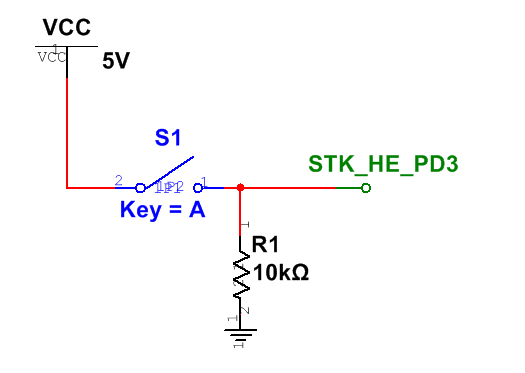
\includegraphics[width=0.5\textwidth]{billeder/BABY_SWITCH}
    \caption{Schematic over knap for lyddetektion}
    \label{fig:BABY_ALARM}
\end{figure}



% Systembeskrivelse

\chapter{Systembeskrivelse (MK)}

Fra kundens synspunkt består systemet af en computer og nogle kontrollerbare stikdåser rundt i huset samt en babyalarm. Her beskrives hele systemet mere detaljeret.

\begin{figure}[H] \centering
\fbox{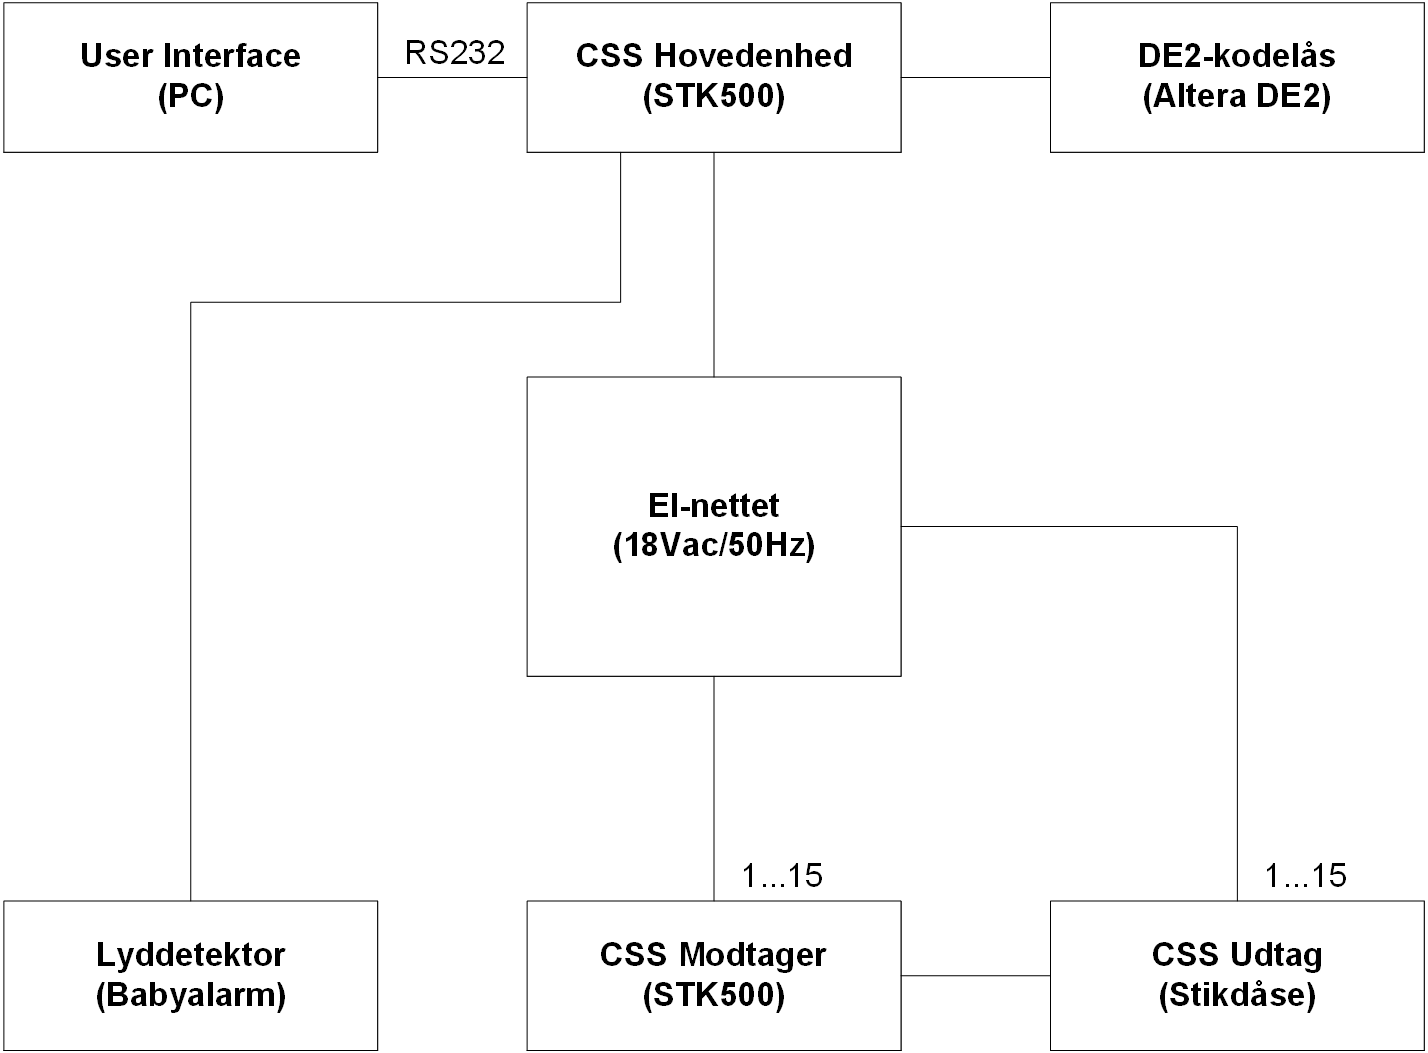
\includegraphics[width=0.65\textwidth]{billeder/diagrammer/Sys_oversigt}}
\caption{Systemoversigt}
\label{fig:sys_oversigt}
\end{figure}

I figur \ref{fig:sys_oversigt} ser man, at systemet består af en PC, der har forbindelse til CSS-hovedenheden; denne er kundens kontrolenhed(User Interface). Her har kunden adgang til et simpelt menusystem, hvori kunden kan kontrollere stikdåserne(X10-udtagene). Der er mulighed for at aktivere, deaktivere eller udlæse status på systemet. Der er endvidere også mulighed for at ændre mobilnummeret til den person, som skal modtage babyalarm-SMS'en. Hele systemet kræver en 3 cifret adgangskode, der indtastes ved hjælp af et eksternt hardwaremodul(DE2-kodelås).

Når en kommando bliver eksekveret i User Interfacet, sendes der data serielt ud via RS232 til CSS-hovedenheden. Denne data bliver encodet til en X10-bitstrøm og sendt ud på el-nettet(18Vac). Denne bitstrøm bliver så aflæst af X10-udtagene, og hvis et X10-udtag har den korrekte adresse, vil kommandoen blive udført på denne.

Babyalarmens funktion er at give CSS-hovedenheden besked om støj i det værelse, hvor lyddetektoren sidder placeret. Lyddetektoren er kablet direkte til CSS-hovedenheden og virker ved, at den ved et givent lydniveau\footnote{se ikke-funktionelle krav i produktdokumentationen} vil sende et signal til CSS-hovedenheden, som via dennes serielle RS232 port fortæller PCen, at der skal sendes en SMS til det forudbestemte mobilnummer med en advarsel.

\subsection*{Installation i hjemmet (PO)}

Her ses, hvordan installationen kunne laves i en kundes hjem. Hængelåsene angiver hvilke enheder i hjemmet, der kan interageres med.

\begin{figure}[H] \centering
\fbox{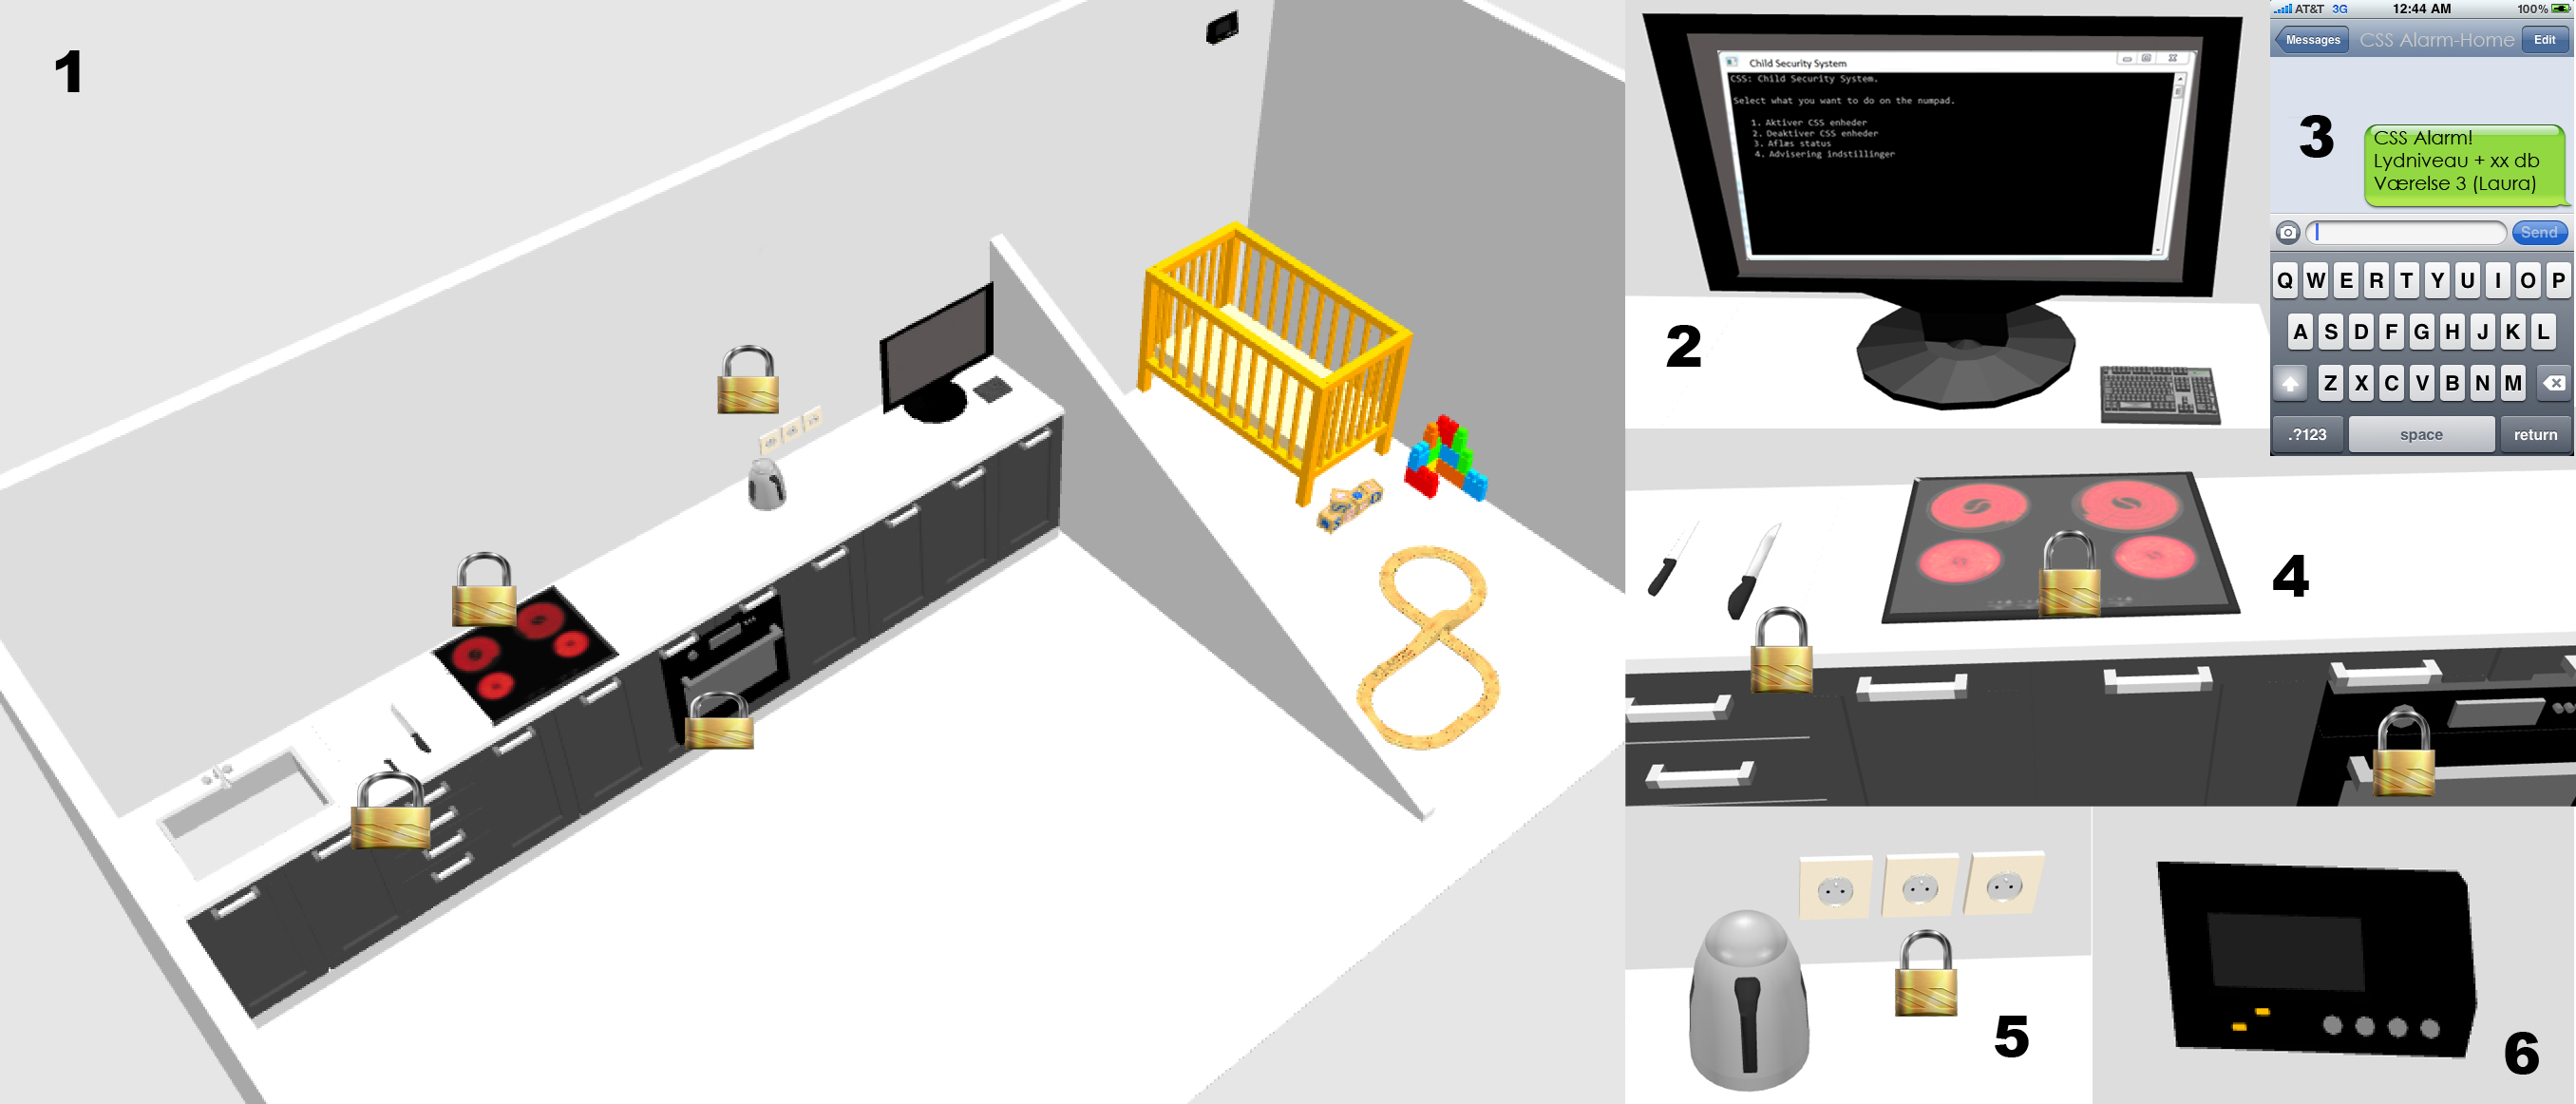
\includegraphics[width=0.65\textwidth]{billeder/Installationsoversigt}}
\caption{Installationsoversigt}
\label{fig:installationsoversigt}
\end{figure}

\begin{enumerate}
\item Samlet oversigtstegning af CSS. 
\item CSS-programmet med tilhørende DE2-kodelås.
\item SMS-besked udsendt af systemet, idet lydniveauet i værelse 3 (Laura) har været over det tilladte.
\item Overblik over, hvad systemet er tiltænkt at børnesikre. Køkken skuffe med skarpe genstande, kogeplader, ovn.
\item 230V udtag. X10 styret, således at det bestemmes, om udtaget skal være aktivt.
\item Babyalarm. Illustrationen vil variere i forhold til virkeligheden.
\end{enumerate}

% Kravspec

\chapter{Krav}
Child Security System er et system vi har udviklet med udgangspunkt i at gøre den almindelige husstand mere sikker for børn. Samtidig skal systemet have en integreret baby overvågning som er tiltænkt som erstatning for den almindelige baby alarm.
Via en hovedenhed styres udvalget enheder, hvorfra disse kan slukkes og og tændes. Disse enheder er almindelige 230 V udtag som ønskes at kunne afbrydes eller syre en magnetlås til aflåsning af døre eller skuffer.

Baby overvågningen består af en sensor der måle lydniveauet i et rum som sender et signal til hovedenheden hvis grænseværdien overskrides. Dette signal fortæller hovedenheden at den skal sende en SMS til et telefonnummer efter kundes ønske.   


% generelle krav for systemet 

\chapter{Kravspecifikation}

\section{Aktører}

\subsection{Bruger}
\begin{table}[htbp] \centering
\begin{tabular}{|p{4cm}|p{7cm}|}
	\hline
\textbf{Aktørnavn} &Bruger \\\hline
\textbf{Type Beskrivelse} &
Bruger aktøren er ejeren af systemet eller den voksne med adgang til Computeren.
Dette kunne være, forældre, barnepige osv.	
\\\hline
	\end{tabular}
\end{table}

\subsection{Barn}
\begin{table}[htbp] \centering
\begin{tabular}{|p{4cm}|p{7cm}|}
	\hline
\textbf{Aktørnavn} &Barn \\\hline
\textbf{Type Beskrivelse} &
Barnet eller børnene i huset, som systemet skal beskytte.	
\\\hline
	\end{tabular}
\end{table}

\subsection{SMS Bruger}
\begin{table}[htbp] \centering
\begin{tabular}{|p{4cm}|p{7cm}|}
	\hline
\textbf{Aktørnavn} &SMS Bruger \\\hline
\textbf{Type Beskrivelse} &
Ligesom Bruger (ejeren, forældrene osv.)
Men kan også være naboen eller et familiemedlem der bor i nærheden.
\\\hline
	\end{tabular}
\end{table}

\section{Usecases}

\subsection{Use Case 1}
\begin{center} \centering
	\begin{longtable}{|p{6cm}|p{8cm}|}
	\hline
		\multicolumn{2}{|l|}{\textbf{UC1: Login}} \\\hline
		\endfirsthead
		
		\multicolumn{2}{l}{...fortsat fra forrige side} \\ \hline 
		\multicolumn{2}{|l|}{\textbf{UC1: Login}} \\\hline
		\endhead		

\textbf{Mål}								
&At Bruger kan logge ind ved hjælp af adgangskode
 \\\hline
\textbf{Initialisering}					
&Bruger vælger login i interface
 \\\hline
\textbf{Aktører og Stakeholders}			
&Bruger(Primær), DE2 Board(Sekundær)
 \\\hline
\textbf{Referencer}						
&Ingen
 \\\hline
\textbf{Antal af samtidige hændelser}	
&1
 \\\hline
\textbf{Forudsætning}					
&At interfacet er tændt
 \\\hline
\textbf{Efterfølgende tilstand}			
&At bruger er logget ind og hovedmenu vises på skærmen. Hele systemet er klar til brug
 \\\hline
\textbf{Hovedforløb}						
& 
\begin{enumerate}

\item Bruger vælger login i interfacet

\item \label{UC2und1}Bruger indtaster 3 koder adskilt af ''Enter'' på DE2 board \newline
\textbf{[Undtagelse \ref{UC2und1}a]} Bruger vælger Annuller

\item Bruger får adgang til hovedmenuen	
 
\end{enumerate}
\\\hline

\textbf{Undtagelser}						
&\begin{enumerate}[label= \ref{UC2und1}a.]
			\item Bruger vælger annuller og kommer tilbage til loginskærm
		\end{enumerate}
\\\hline


		%\textbf{Version}		&1.0 \\\hline
	\end{longtable}
	\label{UC1} 
\end{center}

\subsection{Use Case 2}
\begin{table}[H] \centering
\begin{tabular}{|p{6cm}|p{8cm}|}
	\hline
\multicolumn{2}{|l|}{\textbf{UC2: Deaktiver CSS enhed(er)}} \\\hline
\textbf{Mål}	&
At brugeren kan deaktivere enkelte eller alle enheder, i systemet.
\\\hline
\textbf{Initialisering} &
Bruger trykker "deaktiver", og bliver
præsenteret for hvilke enheder der skal deaktiveres, samt en mulighed for at deaktivere alle
enheder. 
\\\hline
\textbf{Aktører og Stakeholders}	&
Bruger er hovedaktør
\\\hline
\textbf{Referencer} &
Login
\\\hline
\textbf{Antal af samtidige hændelser} &
1
\\\hline
\textbf{Forudsætning} &
At CSS Systemet er helt eller delvist aktiveret.
\\\hline
\textbf{Efterfølgende tilstand} &
Hovedmenu vises
\\\hline
\textbf{Hovedforløb}	&
Bruger trykker deaktiver og følger instruktionerne på skærmen.
\begin{enumerate}
\item Deaktiver alt
\item Deaktiver alle låse
\item Deaktiver babylarm
\end{enumerate}
\\\hline
\textbf{Undtagelser}	&
Ingen
\\\hline
\textbf{Version}		&1.0 \\\hline
	\end{tabular}
	\label{tab:UC2} 
\end{table}

\subsection{Use Case 3}
\begin{table}[H] \centering
	\label{tab:UC3}
\begin{tabular}{|p{6cm}|p{8cm}|}
	\hline
		\textbf{Mål}						&At Bruger kan deaktivere enkelte eller alle enheder, i systemet. \\\hline
		\textbf{Initialisering} 			&Bruger vælger ''Deaktiver'' \\ \hline
		\textbf{Aktører og Stakeholders}	&Bruger(Primær), Eksterne enheder(Sekundær)\\ \hline
		\textbf{Referencer} 				&UC1: Login \\ \hline
		\textbf{Antal af samtidige hændelser} &1 \\ \hline
		\textbf{Forudsætning} 			&Systemet er tændt \\ \hline
		\textbf{Efterfølgende tilstand} 	&Enkelte eller alle enheder er deaktiveret \\ \hline
		\textbf{Hovedforløb}				&

	\begin{enumerate}	
						
					
				\item Bruger vælger ''Deaktiver'' i hovedmenu (UC1 gennemføres)
										
				\item \label{uc3menu}UI viser mulige enheder samt ''Vælg alle'', ''Deaktiver''  og ''Tilbage''
												
				\item Bruger markerer ønskede enheder til deaktivering
												
				\item \label{uc3deact} Bruger vælger ''Deaktiver''\newline
					\textbf{[Undtagelse \ref{uc3deact}a]} Bruger vælger ''Tilbage''
												
				\item \label{uc3sysdeact} Systemet deaktiverer valgte enheder \newline
					\textbf{[Undtagelse \ref{uc3sysdeact}a]} Ingen valgte enheder
				
				\item UI viser besked om at enheder, er deaktiverede
																	
				\item UI returnerer til hovedmenu	
	
	\end{enumerate} \\ \hline

		\textbf{Undtagelser}	
		
		&\begin{enumerate}[label= \ref{uc3deact}a.]
			\item UI returnerer til hovedmenu og UC3 afbrydes
		\end{enumerate}						
							
		\begin{enumerate}[label= \ref{uc3sysdeact}a.]
			\item Hvis ingen enheder er valgt udskrives en fejl på skærmen og beder brugeren om at vælge en enhed og går til UC3.\ref{uc3menu}
		\end{enumerate} \\\hline
											
		%\textbf{Version}		&1.2 \\\hline
		
	\end{tabular} 
\end{table}

\subsection{Use Case 4}
\begin{table}[H] \centering
\begin{tabular}{|p{6cm}|p{8cm}|}
	\hline
\multicolumn{2}{|l|}{\textbf{UC4: Detekter brand}} \\\hline
\textbf{Mål}								&At detektere en opstået brand og eller røgudvikling \\\hline
\textbf{Initialisering}					& CO_2 \\\hline
\textbf{Aktører og Stakeholders}			&Primær: Bruger ønsker at få besked om brand \\\hline
\textbf{Referencer}						& Ingen \\\hline
\textbf{Antal af samtidige hændelser}	& 1 pr. sensor \\\hline
\textbf{Forudsætning}					& CSS sensor aktiv  \\\hline
\textbf{Efterfølgende tilstand}			& Besked til bruger - CSS sensor aktiv \\\hline
\textbf{Hovedforløb}						&  1. CSS sensor aktiv 2. CSS sensor detekterer CO_2  3. CSS sensor udløser alarm (alarm tilstand) 4. Bruger tvinger CSS sensor ud af alarm tilstand\\\hline
\textbf{Tilføjelser}						& Det er muligt at teste sensoren ved at trykke på en knap og herved "illustrere" en brand  \\\hline
%\textbf{Datavariationsliste}			&Test \\\hline
	\end{tabular}
	\label{UC4} 
\end{table}

\subsection{Use Case 5}
\begin{table}[H] \centering
\begin{tabular}{|p{6cm}|p{8cm}|}
	\hline
\multicolumn{2}{|l|}{\textbf{UC5: Detekter barn}} \\\hline
\textbf{Mål}								&At detektere om barnet bevæger sig eller græder \\\hline
\textbf{Initialisering}					&Barnet bevæger sig eller græder\\\hline
\textbf{Aktører og Stakeholders}			&Bruger(Primær): Ønsker at kunne overvåge barnet. SMS Bruger(Sekundær): 																	Modtager SMS ved gråd eller bevægelser. Barn(Sekundær): Ønskes overvåget 				 \\\hline
\textbf{Referencer}						&Advisering \\\hline
\textbf{Antal af samtidige hændelser}	&1 \\\hline
\textbf{Forudsætning}					&At CSS er aktiveret \\\hline
\textbf{Efterfølgende tilstand}			&Sensor stadig aktiv \\\hline
\textbf{Hovedforløb}						&\begin{enumerate}
	
				\item Systemet er aktiveret
												
				\item Systemet opfanger bevægelse eller gråd
												
				\item Systemet kalder advisering
								
			\end{enumerate}\\\hline1.
\textbf{Tilføjelser}					&Ingen \\\hline
%\textbf{Datavariationsliste}			&Test \\\hline
	\end{tabular}
	\label{UC5} 
\end{table}

\subsection{Use Case 6}
\begin{table}[H] \centering
\begin{tabular}{|p{6cm}|p{8cm}|}
	\hline
\textbf{Mål} &
Skriv her  \\\hline

\textbf{Initialisering} &
Skriv her  \\\hline
 
\textbf{Aktører og Stakeholders} &
Skriv her  \\\hline

\textbf{Referencer} &
Skriv her  \\\hline

\textbf{Antal af samtidige hændelser} &
Skriv her  \\\hline

\textbf{Forudsætning} &
Skriv her  \\\hline

\textbf{Efterfølgende tilstand} &
Skriv her  \\\hline

\textbf{Hovedforløb} &
\begin{enumerate}

\item Punkt
\item Punkt

\end{enumerate}   
 \\\hline
 
\textbf{Undtagelser} &Ingen \\\hline
		\textbf{Version}		&1.0 \\\hline
	\end{tabular}
	\label{UC6} 
\end{table}

\subsection{Use Case 7}
\begin{table}[H] \centering
\begin{tabular}{|p{6cm}|p{8cm}|}
	\hline
\textbf{Mål} &
Skriv her  \\\hline

\textbf{Initialisering} &
Skriv her  \\\hline
 
\textbf{Aktører og Stakeholders} &
Skriv her  \\\hline

\textbf{Referencer} &
Skriv her  \\\hline

\textbf{Antal af samtidige hændelser} &
Skriv her  \\\hline

\textbf{Forudsætning} &
Skriv her  \\\hline

\textbf{Efterfølgende tilstand} &
Skriv her  \\\hline

\textbf{Hovedforløb} &
\begin{enumerate}

\item Punkt
\item Punkt

\end{enumerate}   
 \\\hline
 
\textbf{Undtagelser} &
Ingen \\\hline

		\textbf{Version}		&1.0 \\\hline
	\end{tabular}
	\label{UC7} 
\end{table}

% Advisering

\subsection{Use Case 8}
\begin{table}[H] \centering
\begin{tabular}{|p{6cm}|p{8cm}|}
	\hline
\multicolumn{2}{|l|}{\textbf{UC8: Login}} \\\hline
\textbf{Mål}								
&At tilmeldt bruger af systemet kan logge ind ved brug af personlig brugernavn og password
 \\\hline
\textbf{Initialisering}					
&Bruger vælger login i interface
 \\\hline
\textbf{Aktører og Stakeholders}			
&Primær: Bruger
 \\\hline
\textbf{Referencer}						
&Ingen
 \\\hline
\textbf{Antal af samtidige hændelser}	
&Der kan fortages ét login ad gangen (sådan skal det formuleres!)
 \\\hline
\textbf{Forudsætning}					
&At interface er online
 \\\hline
\textbf{Efterfølgende tilstand}			
&At bruger er logget ind og hovedmenu vises på skærmen. Hele systmet er klar til brug
 \\\hline
\textbf{Hovedforløb}						
& 
\begin{enumerate}

\item Bruger vælger login i interface

\item Bruger indtaster personlig brugernavn og adgangskode

\item Systemet validerer brugernavn og adgangskode (Extension 1: Ikke valideret)

\item Bruger får adgang til hovedmenu
 
\end{enumerate}
\\\hline

\textbf{Tilføjelser}						&
ingen \\\hline
%\textbf{Datavariationsliste}			&Test \\\hline
	\end{tabular}
	\label{UC8} 
\end{table}


% Arbejdsprocessen

\chapter{Arbejdsproces}

\section{Udviklingsmodeller}

Metoden vi har arbejdet gennem projektet kommer meget fra den undervisning vi har modtaget i ISE. %tilføj ISE forklarin i ordliste? (indledende system engineering) 
Arbejdsforløbet er bygget op efter v-modellen hvor der først er udarbejde kravspecifikation parallelt med at der er udarbejdet en accepttest og herudfra afvikles resten af processen. v-modellen kan ses illustreret på figur %ref og figur mangler 


\begin{large}
::TODO:: indsæt figur af v-modellen
\end{large}



**** Pouls version

Med udgangspunkt i ISE-undervisningen\footnote{Indledende System Engineering} er projektarbejde opbygget omkring ASE-modellen, se figur \ref{fig:ASE_model}. ASE-modellen er opbygget i 2 faser. En fællesfase og en fagspecifik fase. 


\begin{figure}[htbp]
  \centering
    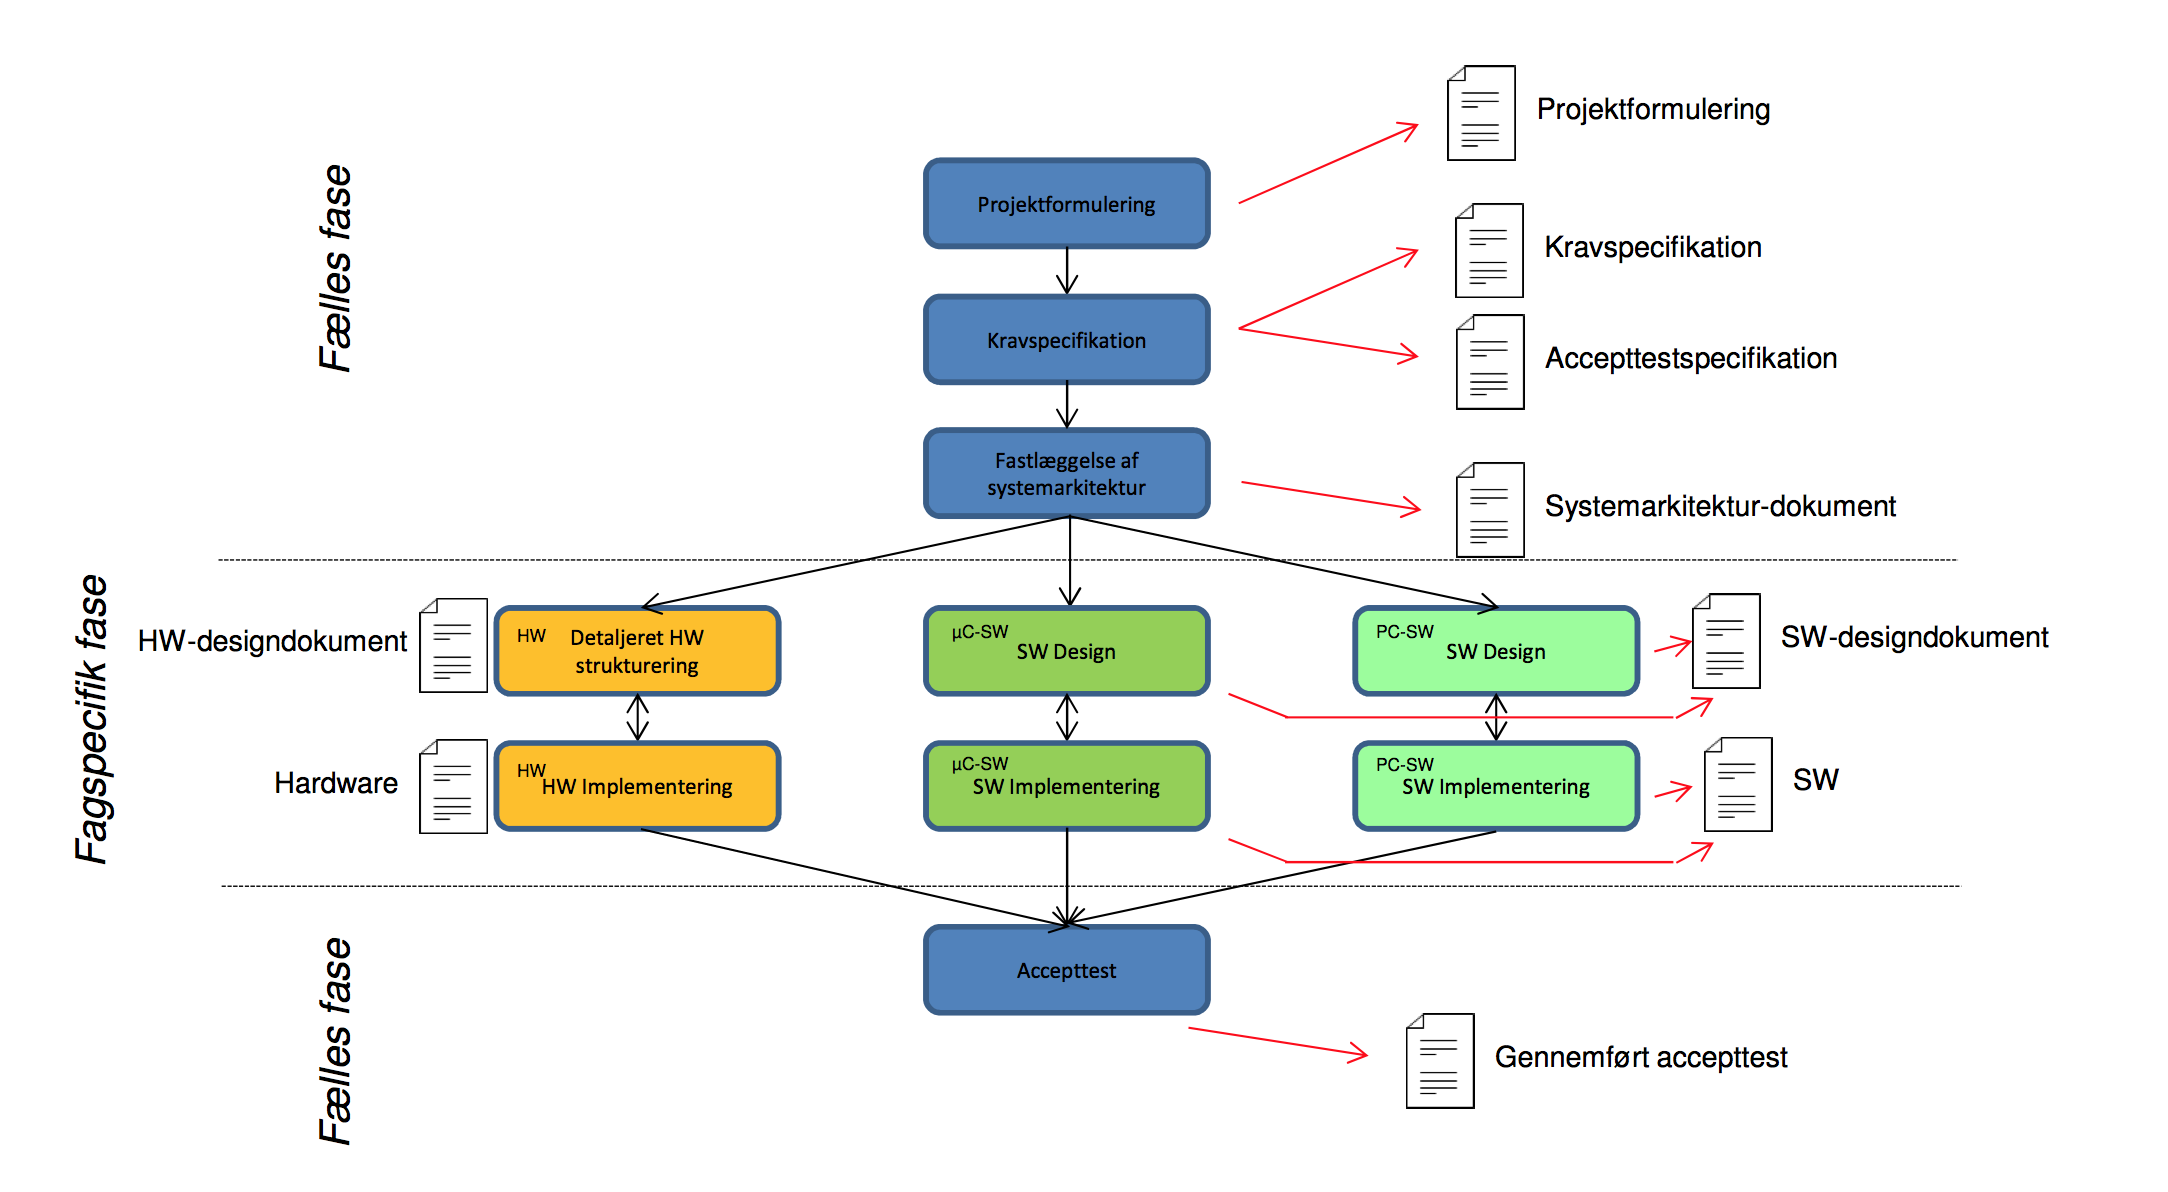
\includegraphics[width=0.8\textwidth]{billeder/ASE-modellen}
    \caption{ASE-modellen}
    \label{fig:ASE_model}
\end{figure}

I fællesfasen arbejde hele gruppen sammen omkring udarbejdelse af de forskellige deldokumenter. 
I den fagspecifikkefase deles gruppen op i mindre teams for at udvikle de fagspecifikke deldokumenter. 

ASE-modellen tager udgangspunkt i V-modellen, se figur \ref{fig:V_model}.   

\begin{figure}[htbp]
  \centering
    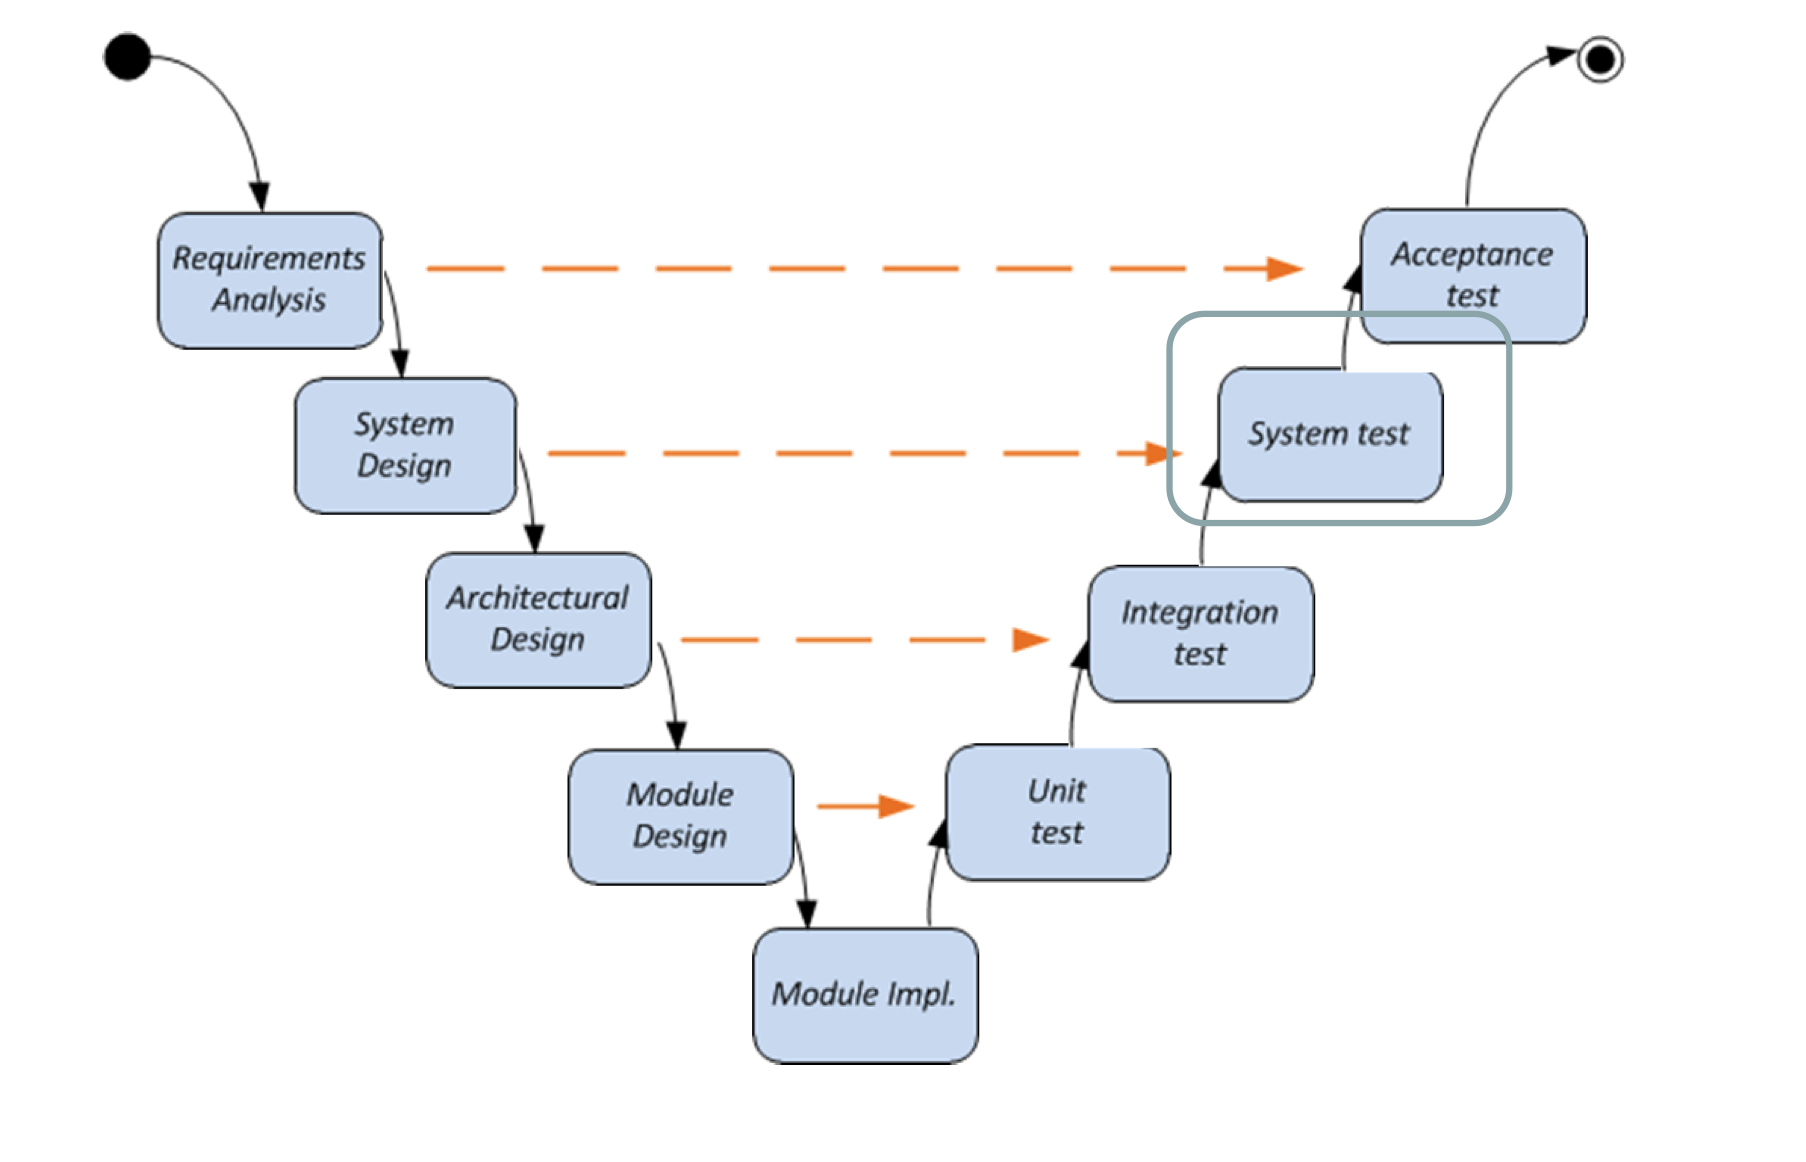
\includegraphics[width=0.8\textwidth]{billeder/V-modellen}
    \caption{V-modellen}
    \label{fig:V_model}
\end{figure}

V-modellen ses på figur \ref{fig:V_model}. Ved at benytte V-modellens opbygning færdiggøres en fase inden en ny påbegyndes. Og ydermere planlægges testen af alle faserne parallelt med at fasen udarbejdes. F.eks udarbejdes acceptesten samtidigt med at kravspecifikationen udarbejdes.  




\section{Møder, tidsplan, logbog og referater}

I forbindelse med projektforløbet er der afholdt en række møder. Vejledermøder, gruppemøder samt reviewmøder.

Vejledermøder er forbindelsen mellem gruppen og gruppens vejleder. Her har det været muligt at få foreløbelig feedback samt et indblik i om det der forventes også er det gruppen forventer. Afholdinngen af vejledermøder har været fastlagt til én i ugen. Det er næsten opretholdt, dog med enkelte aflysninger.

Gruppen har hver uge holdt mindst et, nogle gange flere møder. Disse møder er brugt til at afklare uoverensstemmelser og planlægning af den kommende uge. Under gruppemøderne er der 2 gange brugt tid på en trivsels runde. Her har det været mulgit at give ris/ros til gruppen og eller enkelte. Gruppemøderne startede lidt løst, men dette blev hurtigt ændret til at have en fast mødeholder, som styrede mødets gang. Tidsplanen er under gruppemøderne blevet revideret, således at den altid var opdateret til vejledermøderne.

Gruppekontrakt - bilag - skal underskrives og scannes så?

Reviewmøder har fungere således at gruppen enten udførte review på en anden gruppen og herefter fremlagde dette. Omvendt modtog gruppen lignende review fra andre grupper. Disse review førte ofte til uklarheder, som gruppen herefter måtte tage stilling til i gruppemødet.

Alle møder blev ajour ført med logbog og mødereferat. Her har gruppen haft en fast sekretær. 

\section{HW/SW teams}

\subsection{Hardware teamet}
Hardware teamet bestående af: Jakob, Mick, Poul og Simon har arbejdet meget sammen om opgaven. Samarbejde er nøgleordet for dette team. Alle fire har hovedsagligt arbejdet sammen om hele HW delen. 

\subsection{Software teamet}
I software gruppen bestående af Bjørn, Jeppe og Jesper har vi arbejdet sammen under de indlende faser og først i den detaljerede designfase har vi delt opgaverne op.
Der fra har vi arbejdet individuelt, men dog med regelmæssige møder og afklaringer for at sikre at interface aftaler og ligende stadig blev overholdt.




% Udviklingsværktøjer

\chapter{Udviklingsværktøjer}
Gennem hele projektforløbet er der anvendt forskellige programmer og værktøjer til de respektive opgaver. Nogle programmer havde vi kendskab til på forhånd hvor andre var helt nye for enkelte eller alle gruppemedlemmer.

\section{LaTex og Texmaker (JS, PO)}
Hele rapporten er skrevet i \LaTeX. Dette valg kom i starten af projektet da IDA havde et tilbud om et gratis endags kursus, hvor hele gruppen blev enige om at deltage. 

\LaTeX er et kodebaseret tekstredigerings sprog som er designet netop til større rapporter. Formålet er at gøre forfatteren fri for at skulle bekymre sig om formateringer således at han/hun kan rette al fokus på indholdet i rapporten.

Texmaker er benyttet som teksteditor. Heri er alt \LaTeX koden skrevet. Programmet har indbygget pdf-viewer, der gør det muligt at se det endelige produkt vha. Texmakers kompiler. Texmaker er desuden udstyret med dansk stavekontrol.

Det krævede dog lidt tid i starten at komme i gang med \LaTeX, men da det var på plads fungerede det rigtig godt. 

\section{Microsoft Visual Studio (BS)}
Udviklingsprogrammet Microsoft Visual Studio 2012 er brugt til softwareprogrammeringen til PC.

\section{Atmel Studio (BS)}
Atmel Studio 6.1 er det brugte værktøj til programmering af software til CSS-hovedenheden og X10-udtaget.

\section{National Instruments Multisim (PO)}
National Instruments Multisim er benyttet i forbindelse med design af kredsløbsdiagrammer. 

\section{Microsoft Visio (JS)} % UML & SysML
Som del af ISE-undervisning er der blevet undervist og anvendt Microsoft Visio til udarbejdelse af diverse diagrammer. Herunder UML og SysML. SysML er anvendt til at designe blok- og internalblok-diagrammer for hardwaren. UML er anvendt til klasse- og sekvensdiagrammer. 

\section{Altera Quartus II (PO)}
Altera Quartus II er anvendt til VHDL programmeringen af DE2 kodelåsen.

\section{Electronic ToolBox App (JS)}
Electronic ToolBox er en applikation der er udviklet til iOS. Den indeholder informationer omkring det meste elektronik og værktøjer til diverse udregninger af kredsløbsdesign. Vi har primært anvendt det til udregninger på knækfrekvenser i forbindelse med høj-, lav- og båndpasfiltre.  

\section{Filhåndtering (JS, PO)}
Til håndtering af filer er nedenstående 3 løsninger brugt. 

\subsection{GitHub}
GitHub er et sky-basseret versionsstyringsprogram. Det er brugt til de produktmæssige dokumentationer, dvs. software kode, hardware diagrammer og projektdokumentation samt projektrapporten.

\subsection{Dropbox}
Dropbox benyttes som cloud løsning. Dropbox har fungeret som fælles harddisk. Primært benyttet i forbindelse med de 2. afholdte reviews. Ydermere er dropbox benyttet til deling af litteratur. 

\subsection{Google Drev}
Logbogen og mødereferater er udarbejdet i Google Drevs dokument funktion. Og tidsplanen er udarbejdet i regneark funktionen. På den måde kan alle se og rette i det samme dokument samtidigt. 




% Systemarkitektur

\chapter{Systemarkitektur}

\section{Hardware arkitektur}

Efterfølgende diagrammer viser hvordan hardware arkitekturen er opbygget.\footnote{For yderlige BBD/IBD se projektdokumentation afsnit System Artitektur.}

\begin{figure}[htbp] \centering
\section{Domænemodel}
{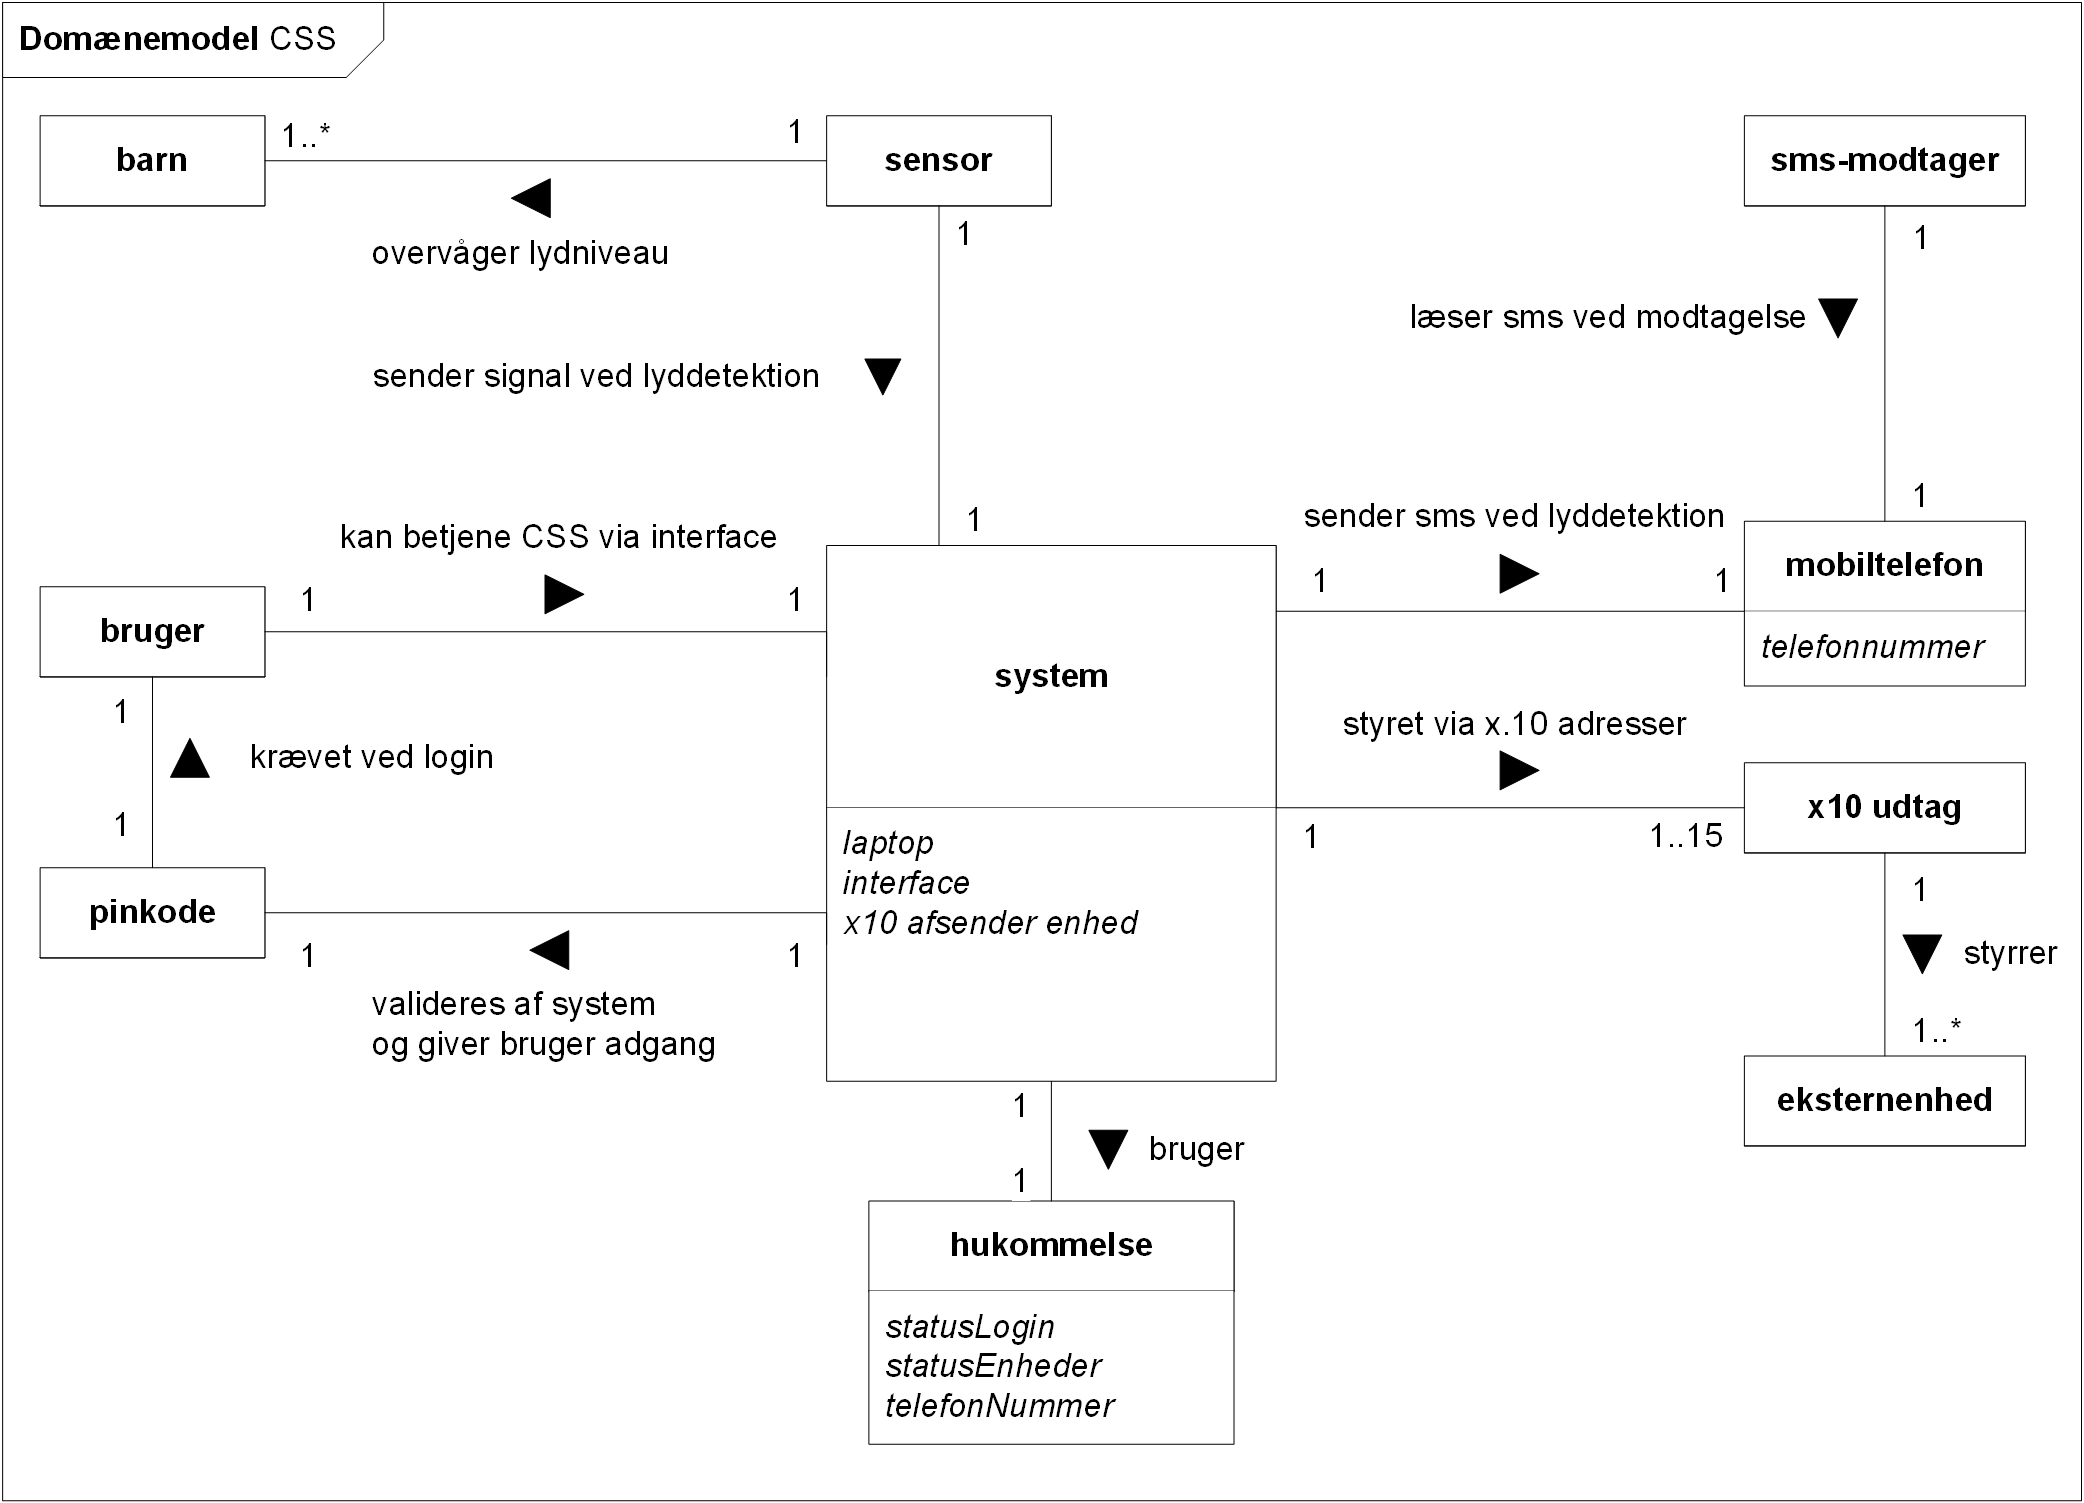
\includegraphics[width=\textwidth]{billeder/diagrammer/Domain_Model}}
\caption{Domænemodel}
\label{lab:domainmodel}
\end{figure}
Domænemodel er udarbejdet i samarbejde med kunden. Denne har til opgave at give et struktureret billede af systemets funktionalitet og sammenhæng. Domænemodellen gør ikke brug af fagudtryk, men pile og kortfattede samt præcise sætninger anvendes for at beskrive sammenhængen mellem blokkene. Dette er med til at opnå en højere forståelse, af systemet som helhed, for kunden.

\newpage

\begin{figure}[!htbp] \centering
\subsection{BDD Hardware}
{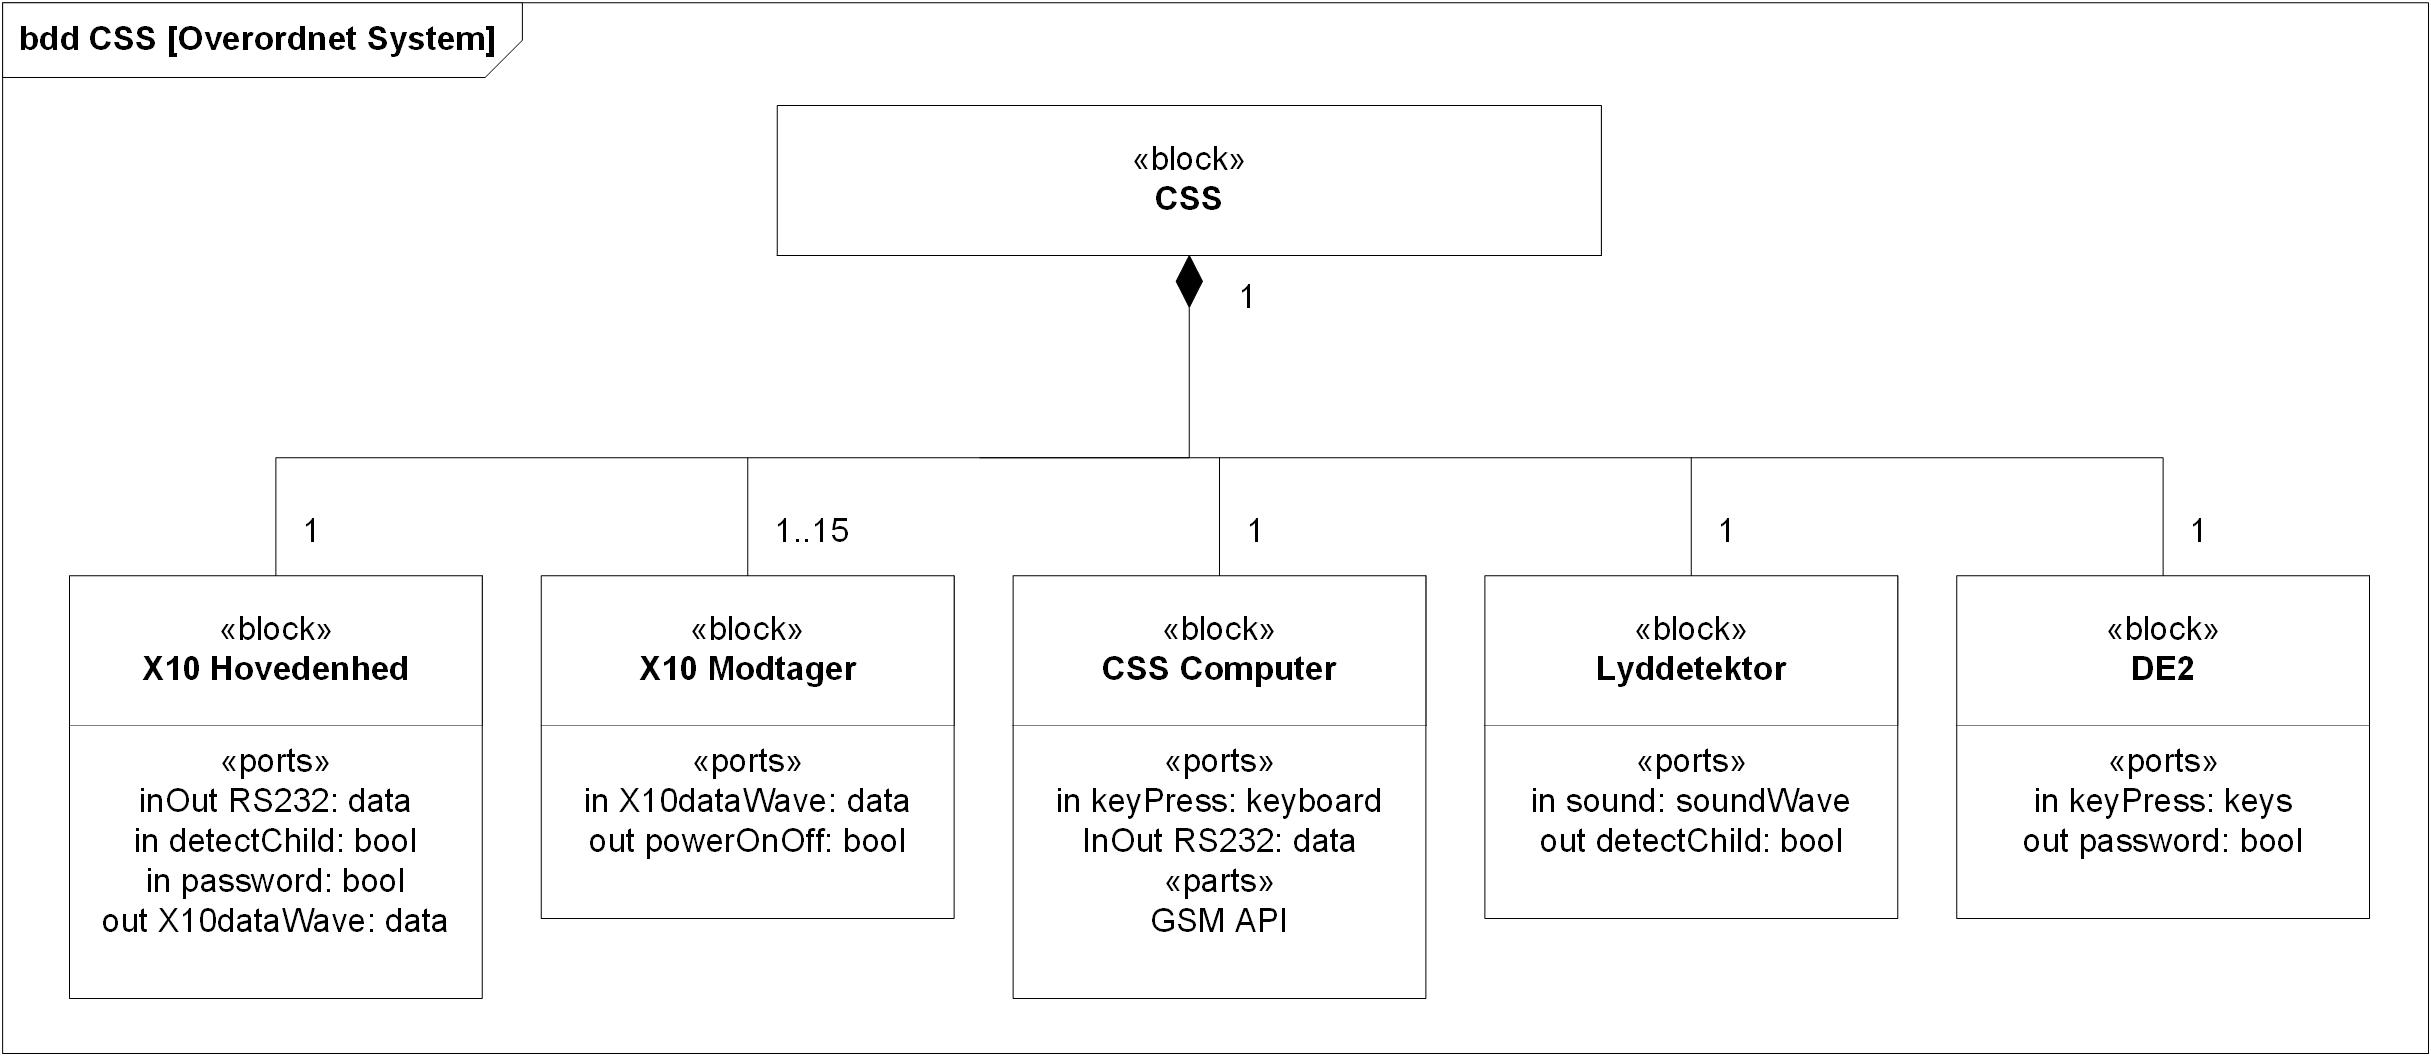
\includegraphics[width=0.9\textwidth]{billeder/diagrammer/BDD_Hardware}}
\caption{BDD Hardware}
\label{lab:bddhardware}
\raggedright
\end{figure}
BDD diagrammet giver et overblik over hvad det samlede system består af. Vi ser en port beskrivelse som viser hvilke signaler hver blok består af.


\begin{figure}[!htbp] \centering
\subsection{Plantegning over HW}
{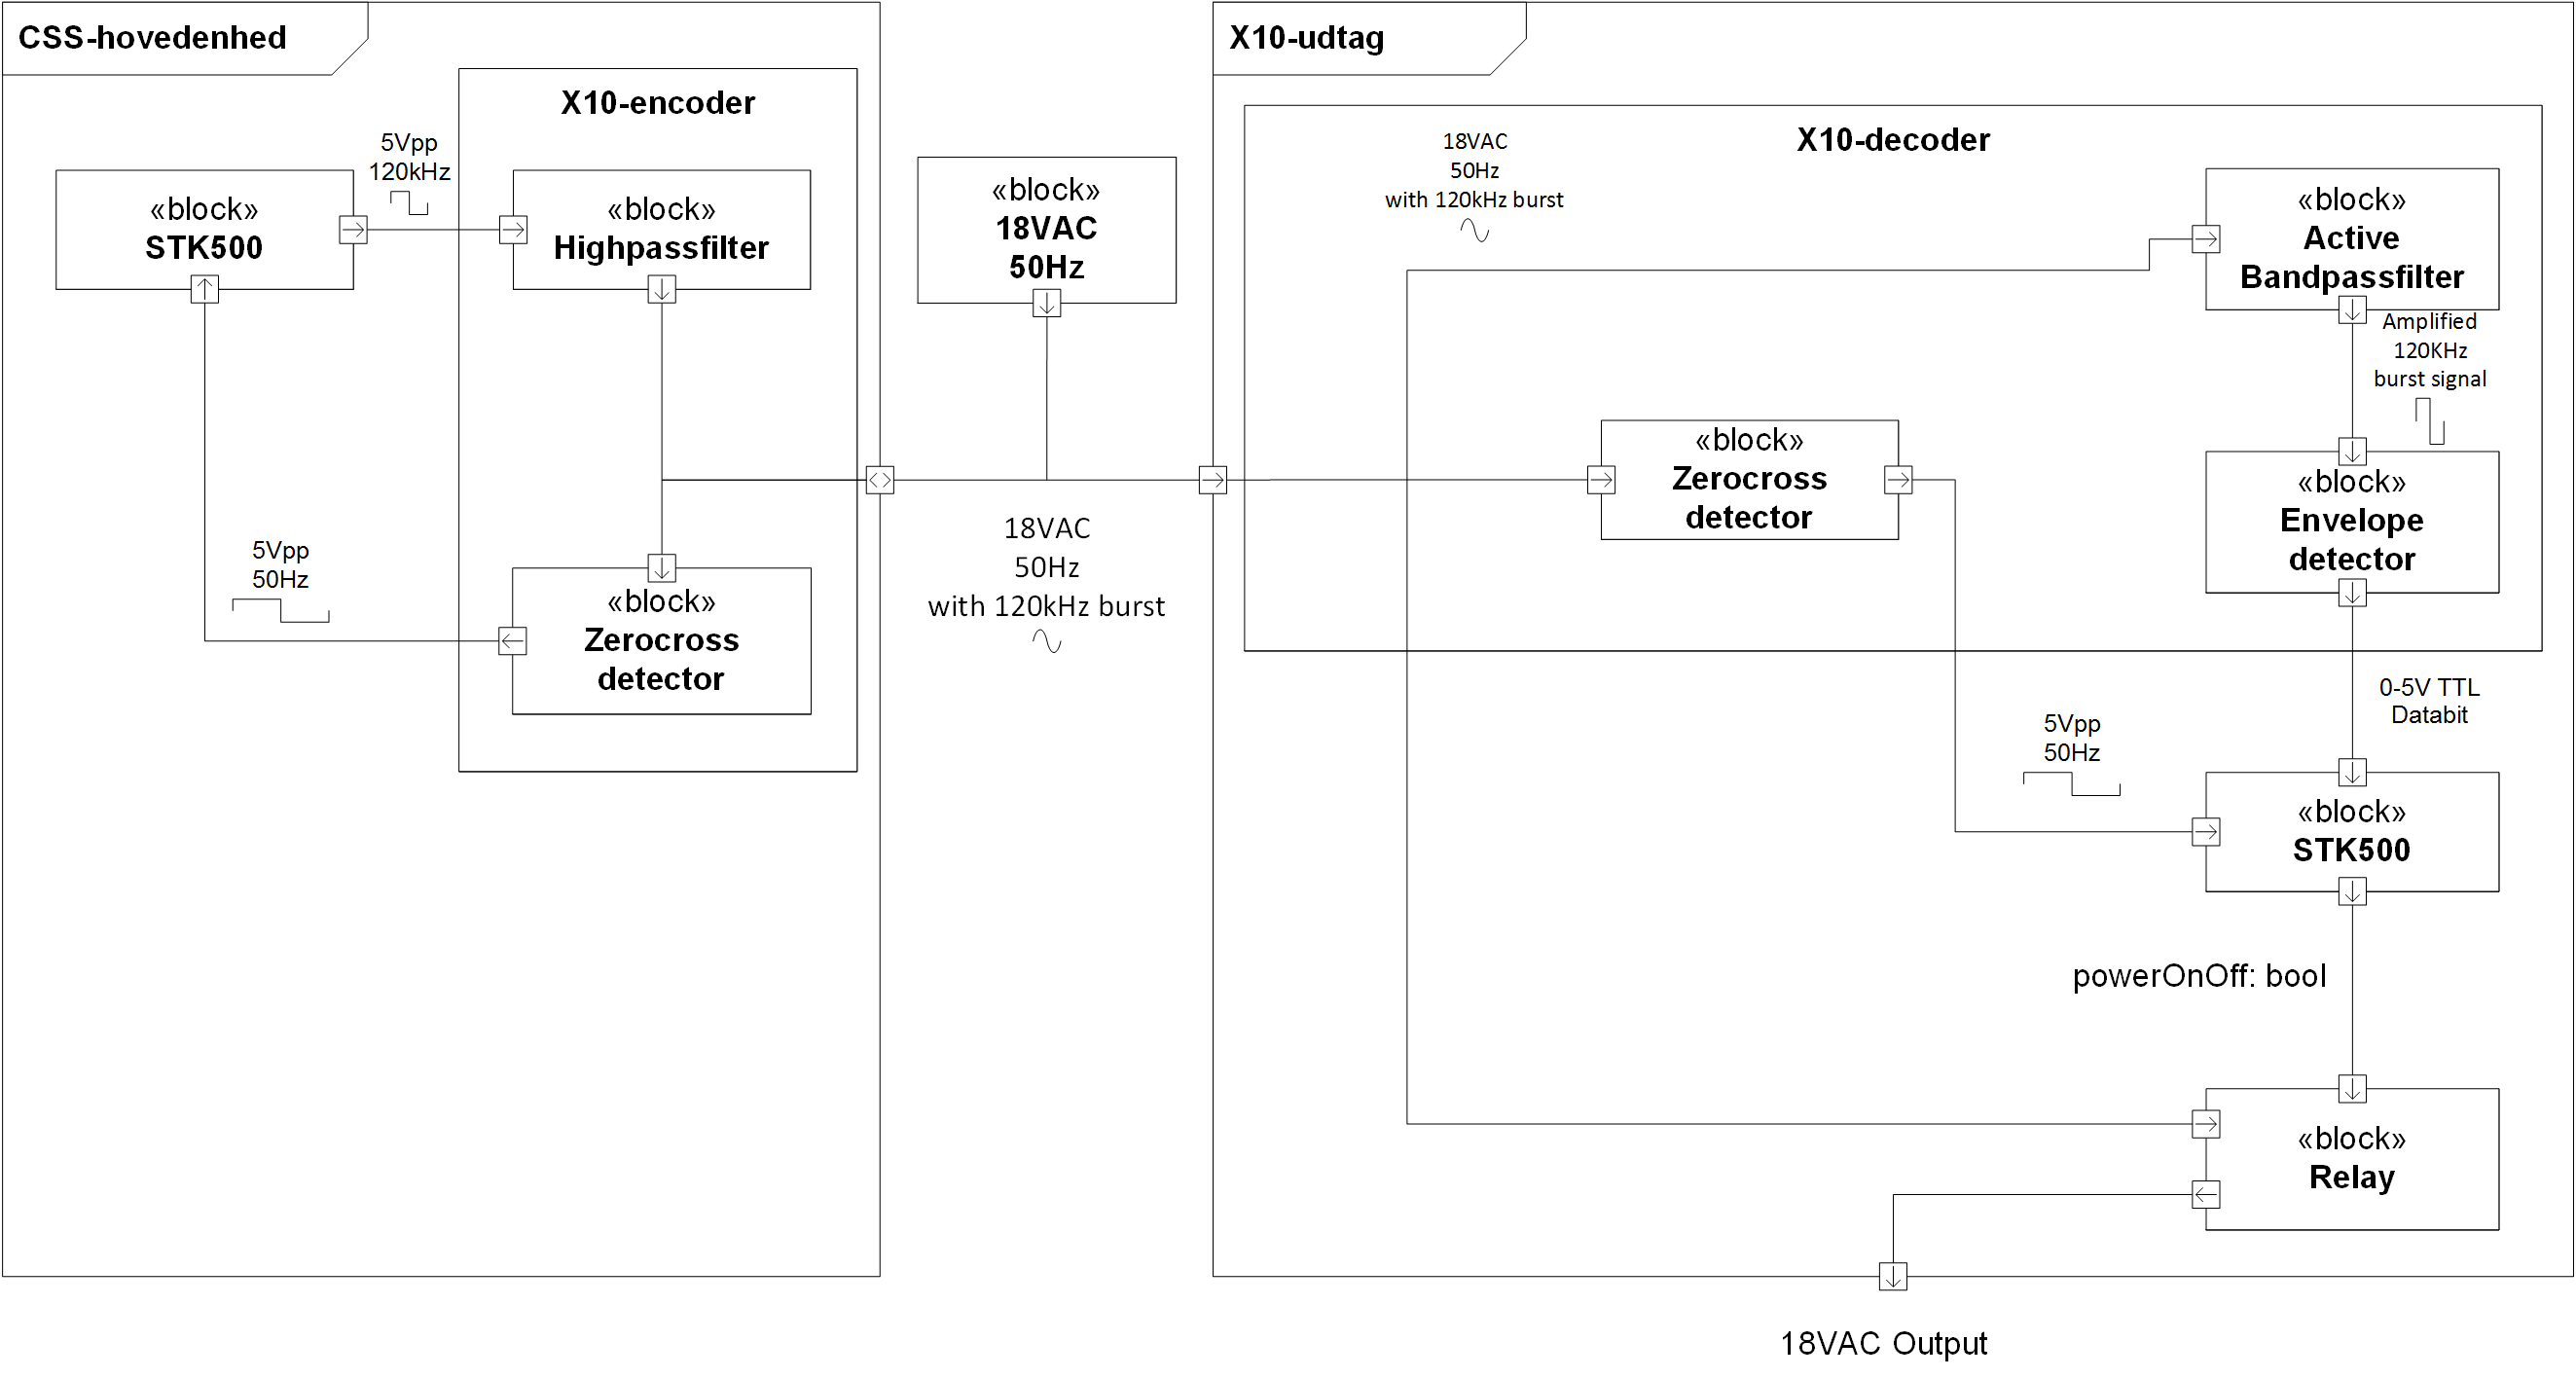
\includegraphics[width=0.9\textwidth]{billeder/diagrammer/Plantegning_over_HW}}
\caption{Plantegning over HW}
\label{lab:Plantegning over HW}
\raggedright
\end{figure}
Plantegningen over HW giver et overblik over hvordan CSS hovedenheden og X10 modtager er forbundet, samt hvilken type signaler der bliver sendt imellem dem.

\clearpage

\section{Software arkitektur}
\subsection{PC}

\subsection{CSS hovedenhed}

\subsection{CSS udtag}


%  Design - sections af HW og SW

\chapter{Design}

% HW

\section{Hardware design}

% HW design


% SW

\chapter{Software design}

\section{Logical View}
\begin{figure}[!htb]
     {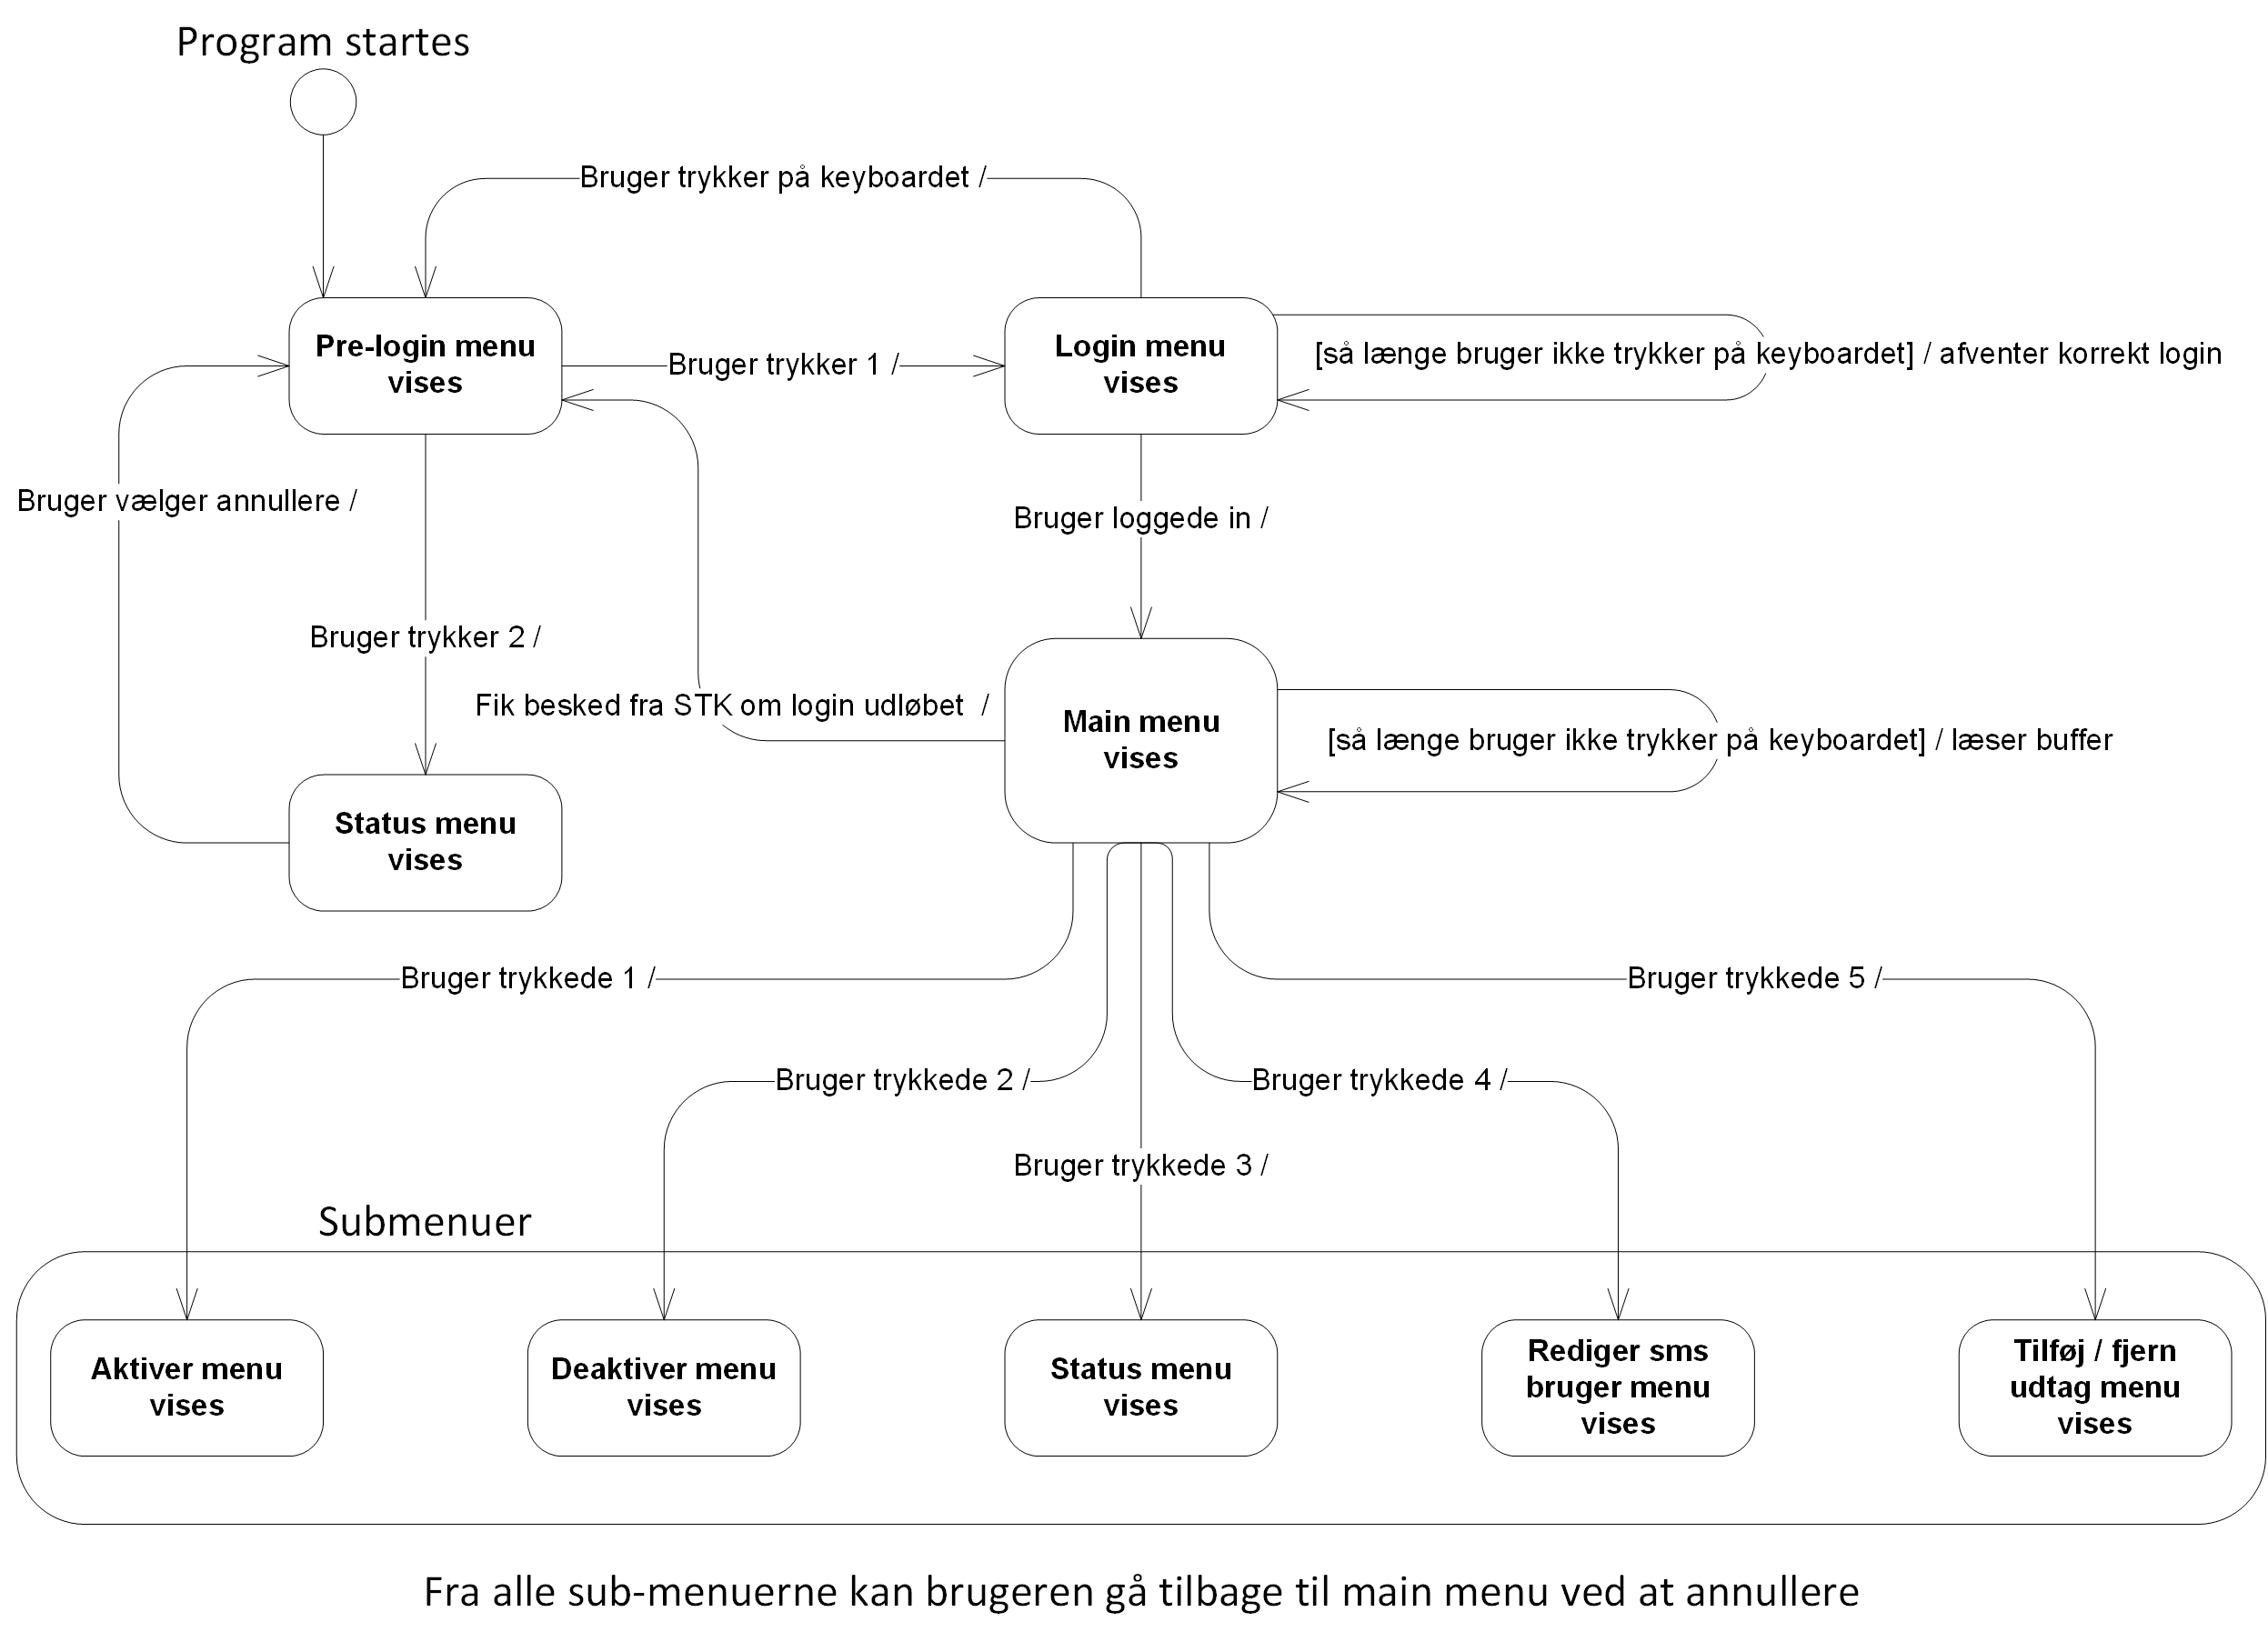
\includegraphics[width=\textwidth]{billeder/uml/state_machine_main}}
     \caption{State machine diagram over forløbet fra PC start til menuer.}
     \label{fig:State_machine_pc}
\end{figure}

Diagrammet ovenfor skal illustrere hvordan forløbet er fra PC opstart. Hvor man møder Pre-login menuen som kun giver en mulighed for at få vist login menu eller vis status menu. Efter der er logget ind vil den stå og føle på input bufferen, på den port hvor PC'en er forbundet med CSS hovedenheden. Det gør den for at en evt. babyalarm kan afbryde forløbet og blive sendt. Desuden kan CSS-hovedenheden give besked om at der ikke længere er logget ind, hvilket sender brugeren til pre-login menuen igen.

\medskip

Når brugeren så trykker på en tast og trykker enter vil han blive sendt til en af de 5 menuer. Dog stadig under forudsætning af at han valgte en værdi imellem 1-5 for den pågældende menu. Ved forkert tast sker der ingenting. Fra hver af de 5 sub-menuer har Brugeren mulighed for at annullere og komme tilbage til main menuen. Dette gør denne ved at taste 27 og enter.


\clearpage

\begin{figure}[!htb]
     {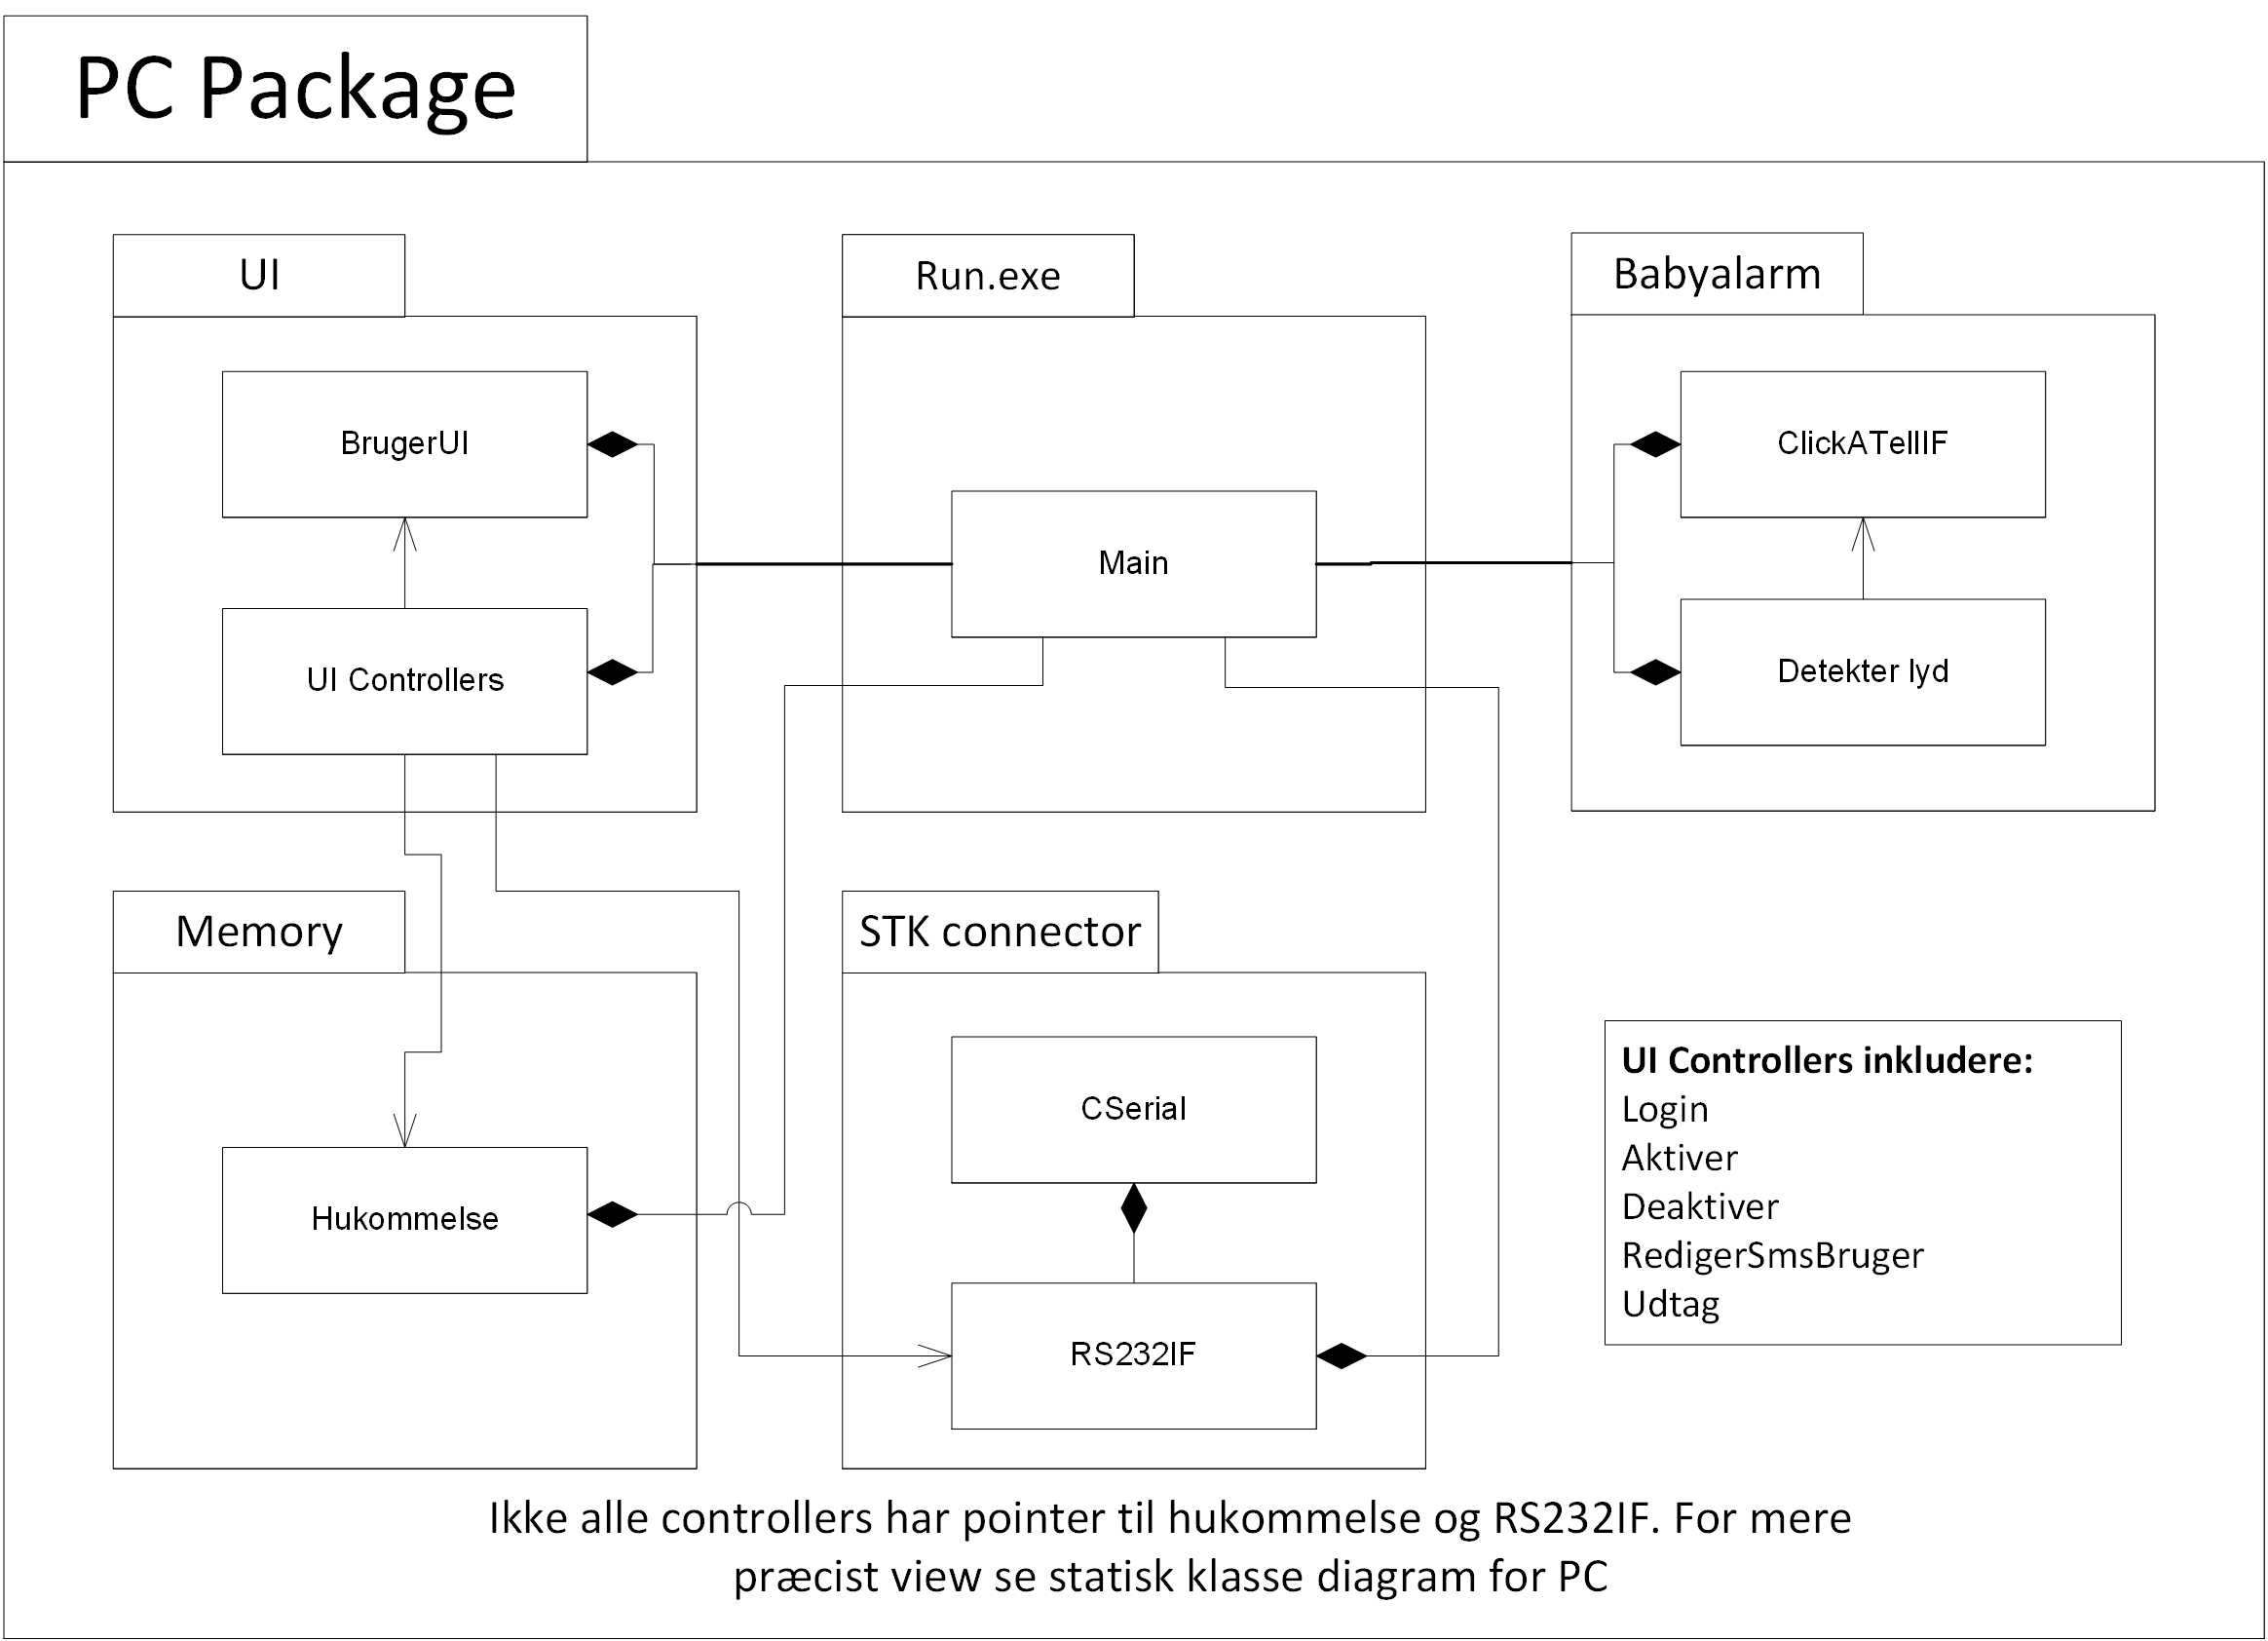
\includegraphics[width=\textwidth]{billeder/uml/logical_view_pc}}
     \caption{Logical view: PC package}
     \label{fig:PC_package}
\end{figure}

Figuren ovenfor viser de forskellige pakker man kan indlede PC klasserne i. Alle controllers som har UI pointers er smidt i UI pakken sammen med BrugerUI. STK Connector pakken indeholder RS232IF og så har den et CSerial \footnote{CSerial klassen er fra http://www.codeguru.com/. Klassen og den fulde URL adresse ligger desuden på CD'en i Reference mappen} objekt som er en klasse der har de 5 mest basale metoder til at sende og læse på en seriel port.


\clearpage

\begin{figure}[!htb]
     {\includegraphics[width=\textwidth]{billeder/uml/logical_view_CSS_Hovedenhed}}
     \caption{Logical view: CSS Hovedenhed package}
     \label{fig:CSS_Hovedenhed_package}
\end{figure}

Figuren ovenfor viser de forskellige pakker man kan inddele CSS hovedenheds klasser i.

% CircBuffer
\subsection{Klasse CircBuffer (BS)}
Efter som X10 kommunikationen er meget langsom (50 bits/s) bruges en buffer til at holde på kommandoerne ind til de er klar til at blive afsendt. Dette er CircBuffer klassens opgave.
Denne er udformet som en cirkulær buffer som kan holde 2 fulde kommandoer. Bemærk at i følge X10-protokollen skal alle kommandoer afsendes to gange. Så der er plads til 4 kommandoer, hvor to af dem altid er de samme.

Klassen er bygget til selv at holde styr på hvilket bit der skal sendes næste gang. Dette forenkler brugen væsentligt, da udtagning af data fra bufferen sker fra en interrupt service rutine (ISR). Denne rutine er beskrevet i detaljer senere.

Alle kommandoer termineres med '\textbackslash 0' karakteren. 

% X10IF klasse design
\subsection{Klasse X10IF (BS)}
En af de kritiske og avancerede klasser er X10IF klasserne på hhv. CSS-hovedenheden og X10 Udtaget. I designfasen er der udviklet sekvensdiagrammer som beskriver nogle af metoderne og sammenspillet til andre klasser.

Funktionaliteten for metoden sendKommando() i X10IF klassen, på CSS-hovedenheden, har som ansvar at afsende en fuld X10-kommando, iht. protokollen, ud fra en parameter formateret som vist i tabel \ref{table:X10_sendKommando_format}.

\begin{table}[h]
	\caption{Parameter opbygning til sendKommando() metoden i X10IF}
	\centering
	\begin{tabular}{|c|c|c|}
		\hline 
		\textbf{Byte} & 0 & 1..4 \\ \hline
		\textbf{Data} & Kommando & Adresse \\ 
		\hline 
	\end{tabular} 
	\label{table:X10_sendKommando_format}
\end{table}

Metoden skal først omskrive den modtagende kommando til en X10 bit streng. Her efter indsættes alle bit's i en buffer, hvorfra de afsendes når der detekteres et zero cross. 
Sekvensen er vist i figur \ref{fig:X10_sendKommando_sd}.

\begin{figure}[!htb]
     {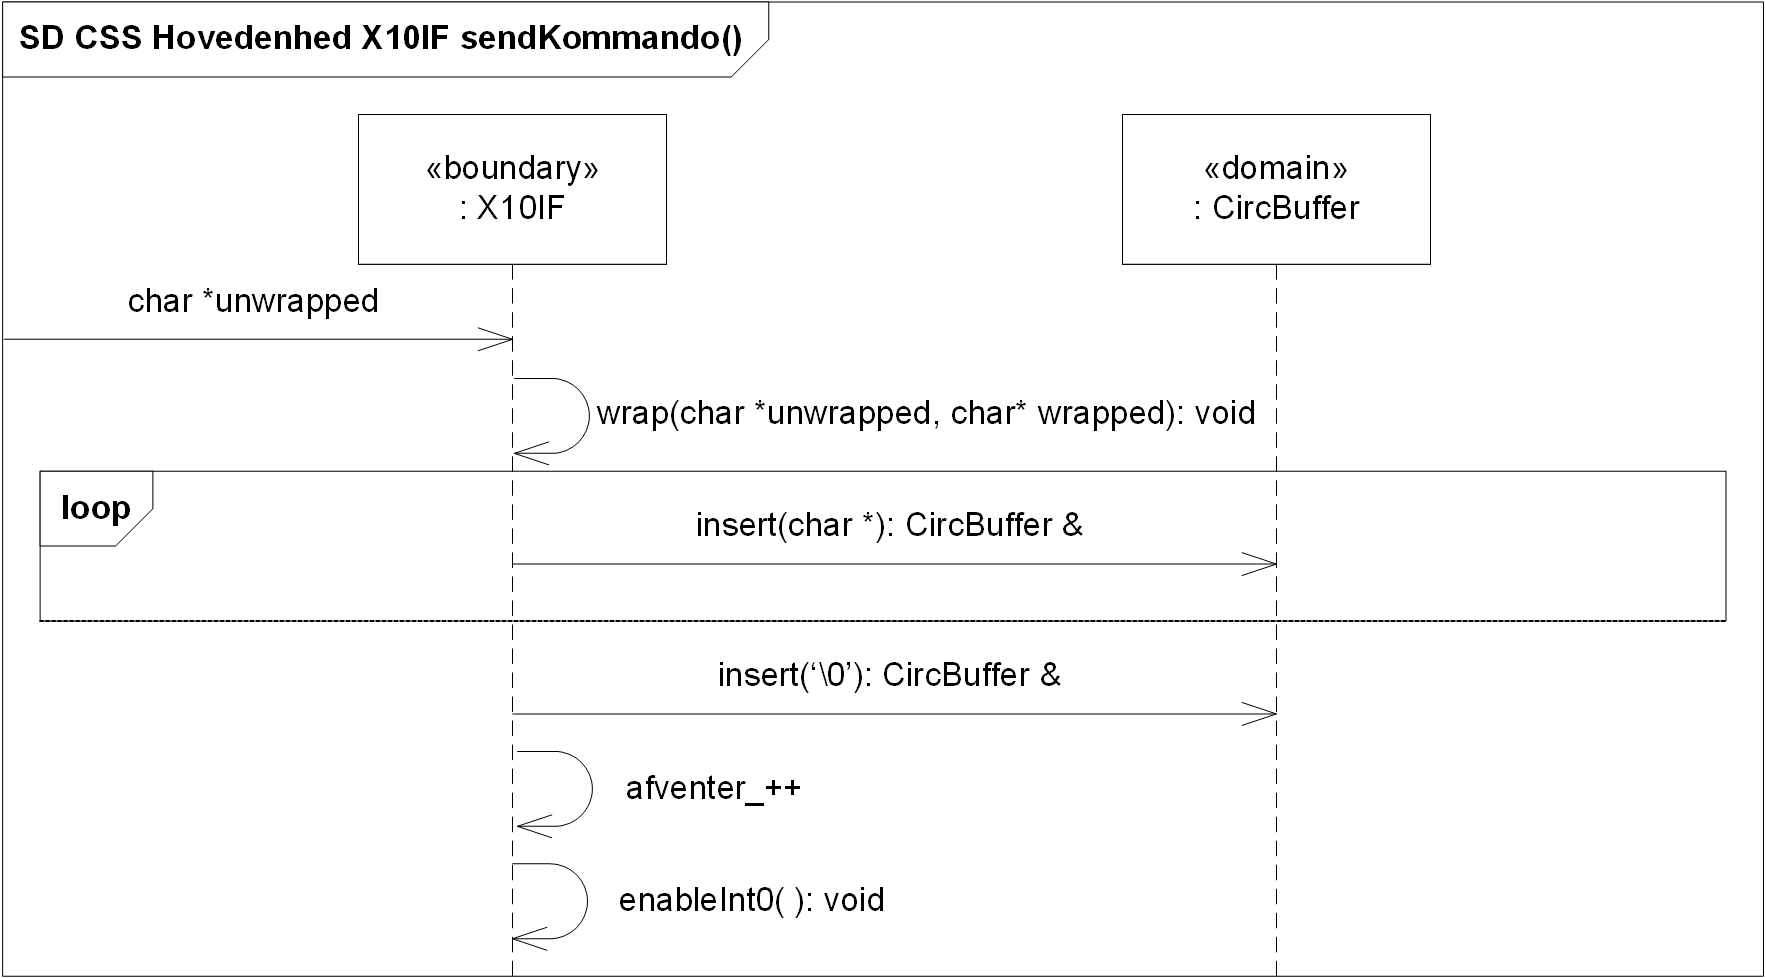
\includegraphics[width=\textwidth]{billeder/uml/CSS_X10IF_sendKommando_SD}}
     \caption{Sekvensdiagram for metoden sendKommando() i X10IF klassen på CSS hovedenheden}
     \label{fig:X10_sendKommando_sd}
\end{figure}

% ZeroCrossInt ISR
\subsection{ZeroCrossInt funktion (BS)}
I tilfælde af et interrupt signal på INT0 benet på CSS-hovedenheden køres en bestemt funktion i microcontrolleren. Dette er kaldet en ISR. Forløbet for denne er beskrevet i sekvensdiagrammet på figur \ref{fig:ZeroCrossISR}.
Først kontrollerer den om der er nogle kommandoer i kø. Der efter henter den det næste bit der skal afsendes fra bufferen. Ud fra værdien bestemmer den om der skal tændes for 120 kHz frekvensen i timeren. Når en kommando er helt sendt nedskriver den køen og hvis køen er tom slår den interruptet fra.

\begin{figure}[!htb]
     {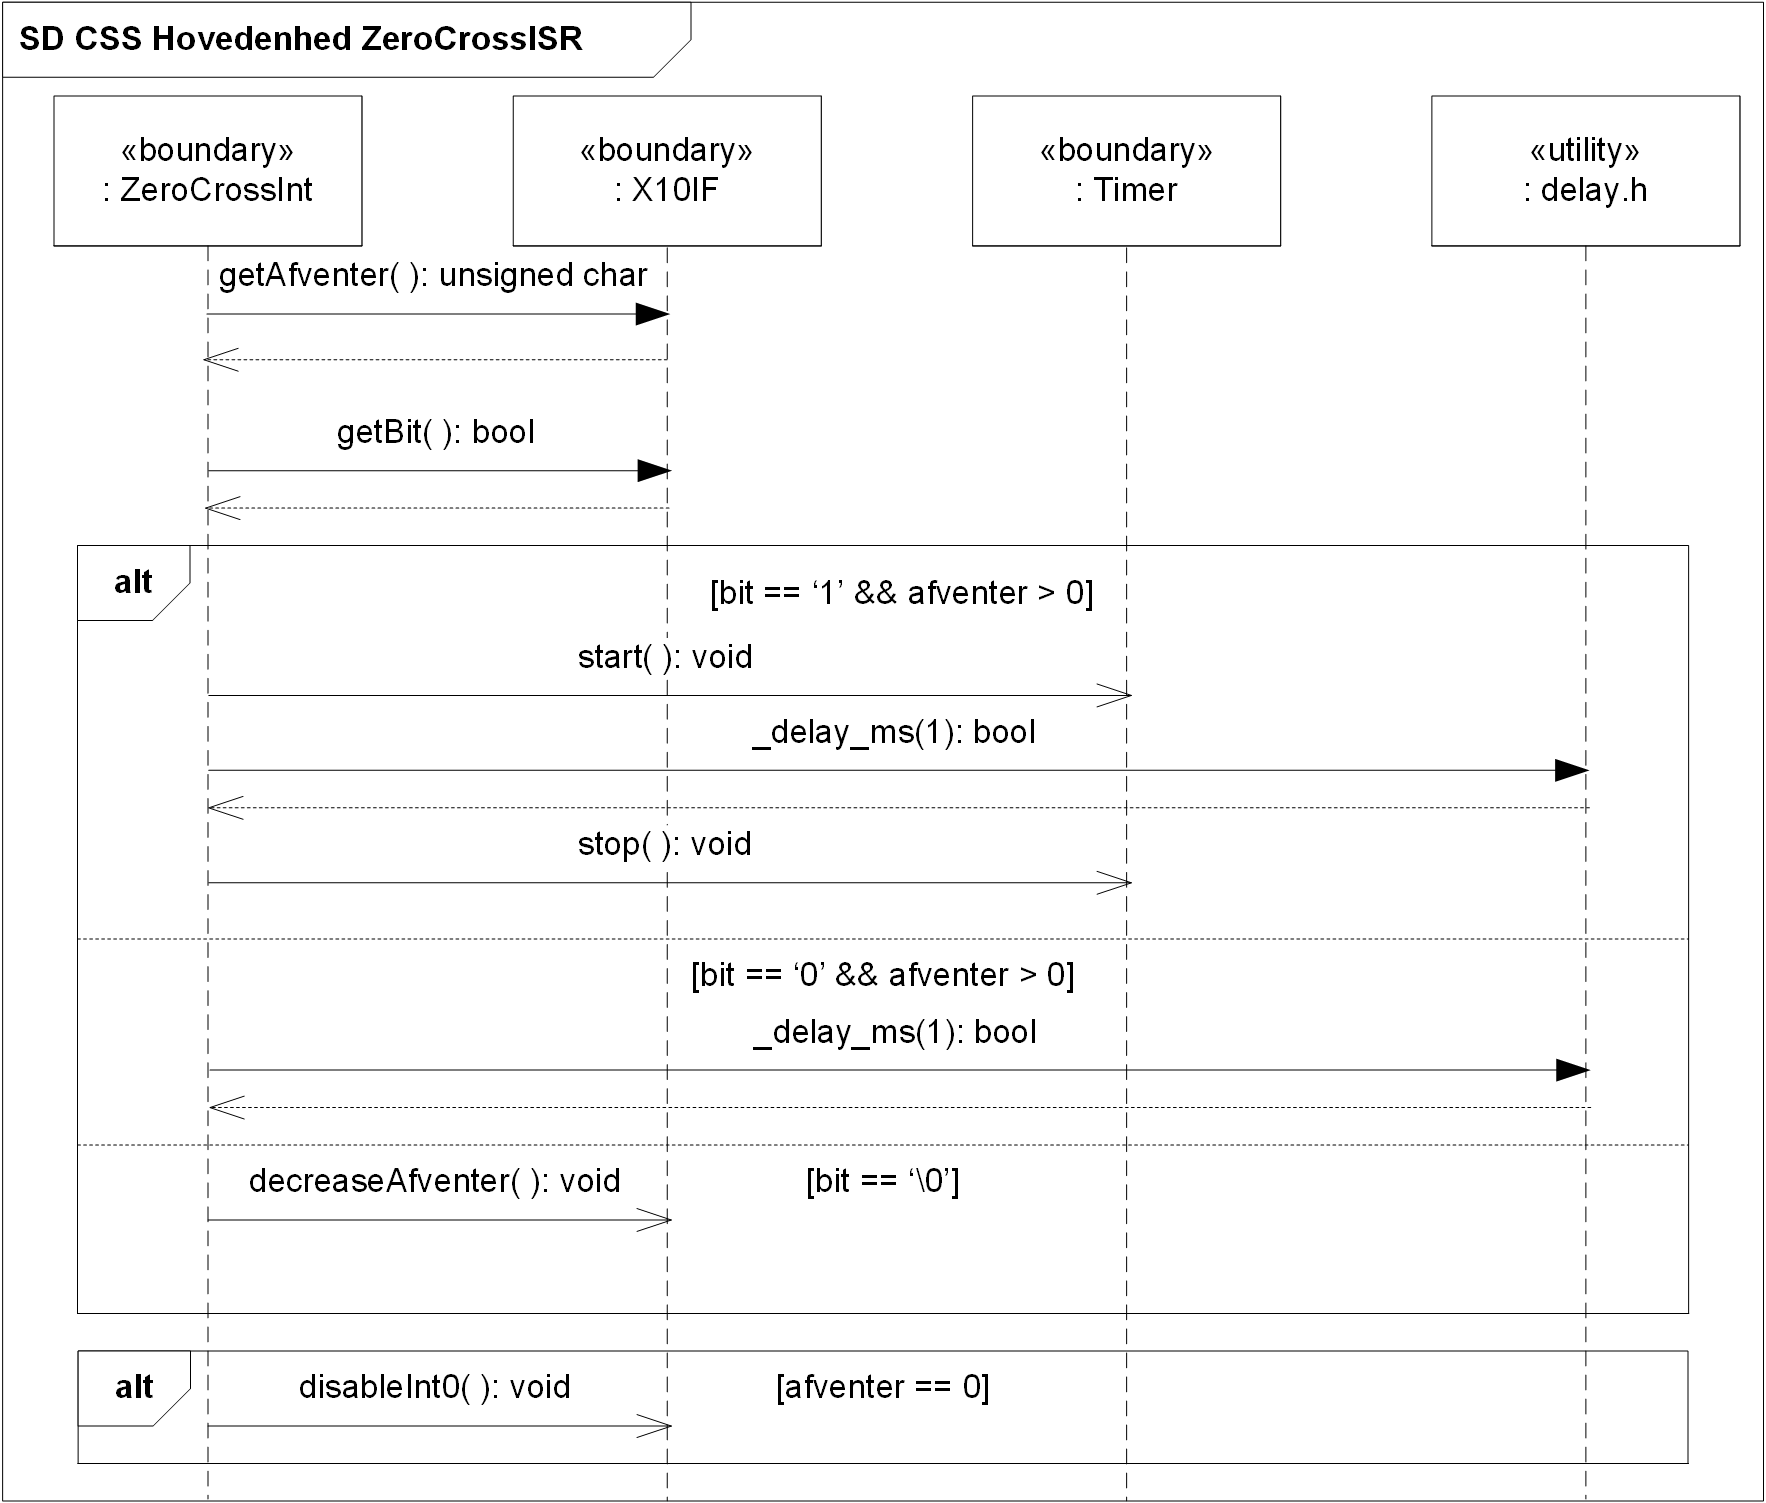
\includegraphics[width=\textwidth]{billeder/uml/CSS_ZeroCrossInt_SD}}
     \caption{Sekvensdiagram for INT0 ISR på CSS hovedenheden}
     \label{fig:ZeroCrossISR}
\end{figure}

% ClickATell
\subsection{Klasse ClickATell (BS)}
For at kunne afsende SMSer i tilfælde af babyalarm bruges en API som kan afsende beskeder via internettet.
ClickATell\textsuperscript{\circledR}\footnote{Online SMS service: http://www.clickatell.com/} er en online service som kan afsende SMSer til et valgfrit telefonnummer ved at kalde en URL adresse.
Ved at bruge Microsoft Windows Shell API\footnote{Microsoft MSDN: http://tinyurl.com/d99m9dz} er det muligt at starte applikationer fra Windows miljøet. Dette bruges til at starte et Internet Explorer-browservindue med en predefineret URL adresse som skaber forbindelse til ClickATell\textsuperscript{\circledR} APIen. 

% Klasse X10IF (udtag)
\subsection{Klasse X10IF (udtag)}
Metoden dekoder den modtaget X10 formateret kommando og adresse. Herefter sendes adressen via en aktiver eller deaktiver.
Sekvensen kan ses i figur \ref{fig:X10-Udtag_unwrapX10Array_SD}.

\begin{figure}[!htb]
     {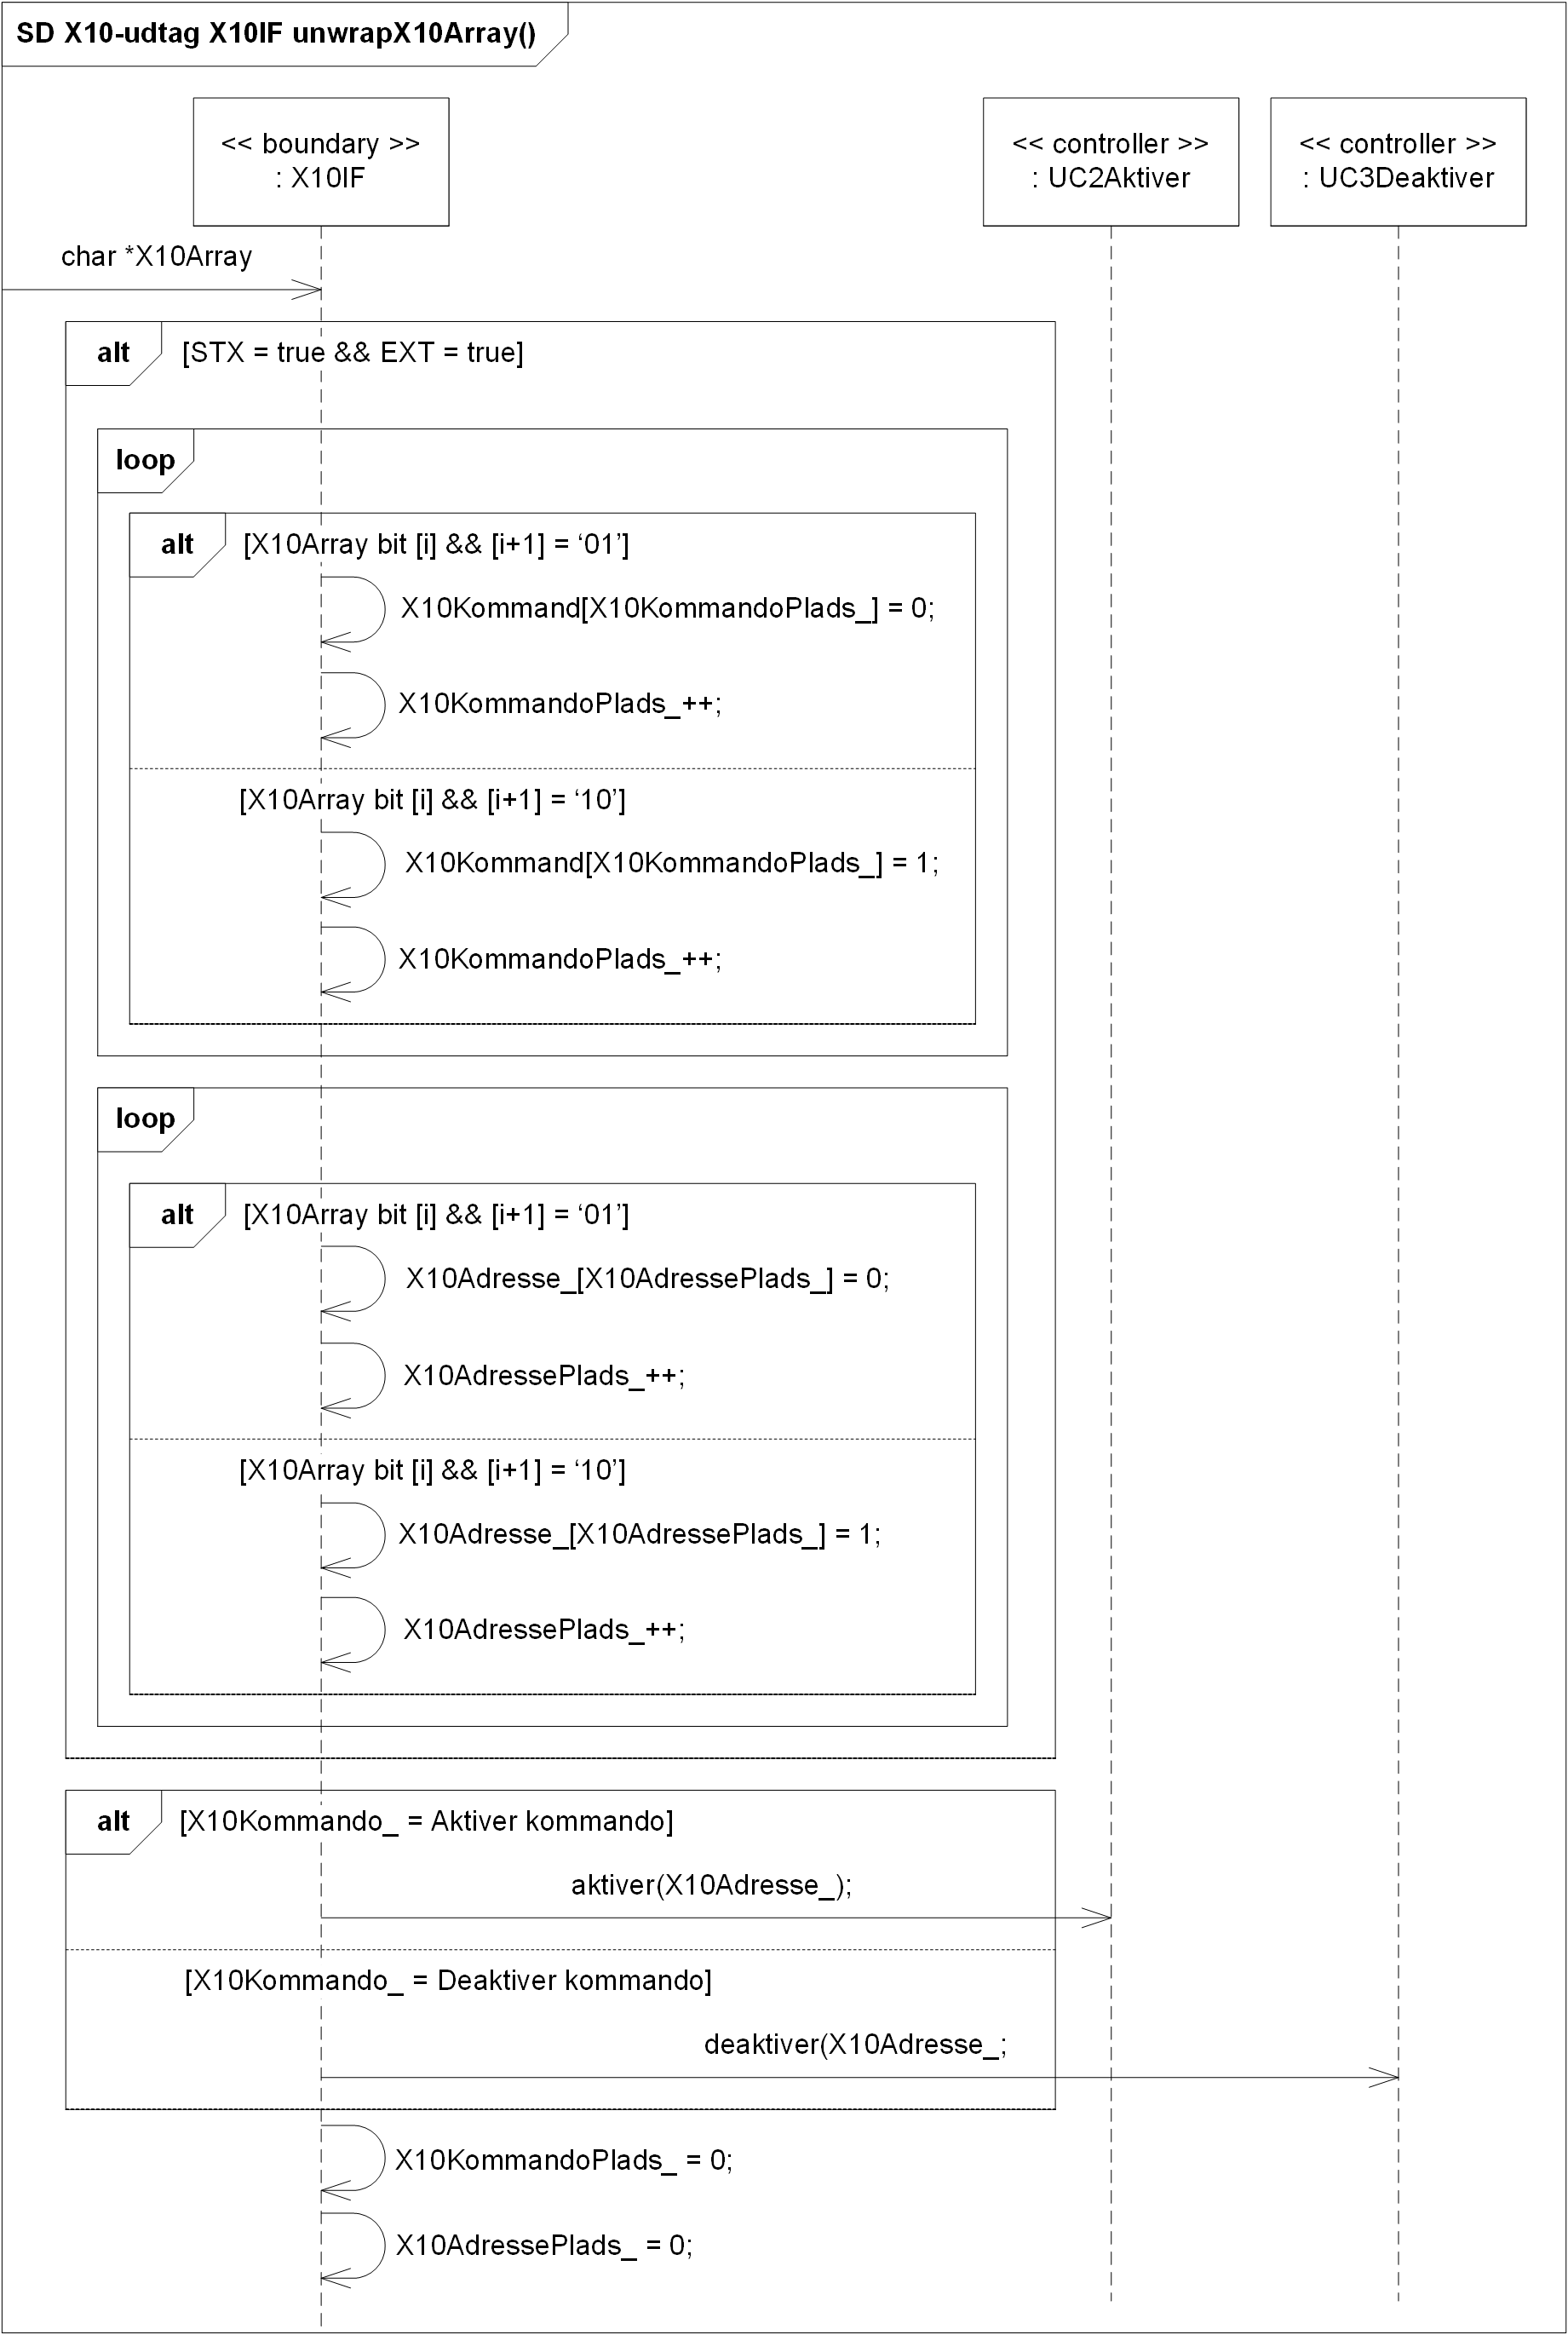
\includegraphics[width=\textwidth]{billeder/uml/X10-Udtag_unwrapX10Array_SD}}
     \caption{Sekvensdiagram for metoden unwrapX10Array() i X10IF klassen på X10-udtaget}
     \label{fig:X10-Udtag_unwrapX10Array_SD}
\end{figure}


\clearpage

\section{Deployment View}

\begin{figure}[!htb]
     {\includegraphics[width=\textwidth]{billeder/uml/deployment_model}}
     \caption{Deployment View}
     \label{fig:Deployment model}
\end{figure}

Deployment view ovenfor illustrere forbindelserne imellem vores enheder og hvor de forskellige software packages er placeret.

\begin{figure}[!htb]
     {\includegraphics[width=\textwidth]{billeder/uml/CSS_Hovedenhed_modtager_deployment}}
     \caption{IBD Deployment View for CSS Hovedenhed og modtager }
     \label{fig:IBD Deployment model}
\end{figure}

Figuren ovenfor viser præcist hvor CSS Hovedenhed package og CSS Modtager package er placeret. De packages kan ses under Logical View. PC Package er placeret på den PC som er koblet til CSS Hovedenheden via RS232 kabel.

\clearpage

\section{Data view}
Vi valgte at vores system skal kunne klare at blive slukket og tændt uden at det ville miste alle data omkring vores udtags tændt/slukket status, adresser, navne og brugeren telefonnummer. Derfor besluttede vi at vi skulle have en klasse på PCen som kunne gemme og loade disse dataer. Det står klassen Hukommelse for.
\medskip

Klassen hukommelse læser og redigere i en text fil hver gang der sker ændringer. Når den læser text filen skriver den hver linje ind på en plads i en vector som kan indeholde strings. Linje 1 i text filen kommer altså til at stå på plads nr 0 i vectoren osv.

\medskip
Telefonnummeret står altid på den første linje i text filen og ligger altså altid på plads nr 0 i vectoren. Enhederne har 3 parametre som vi gerne vil gemme. Deres adresse, navn og status. De bliver gemt i den ordre, dvs at adressen på den første enhed ligger på plads nr 1 (vectornavn[1]) hvorefter navn står på nr 2 og status på nr 3.\\

\begin{figure}[!htb]
     {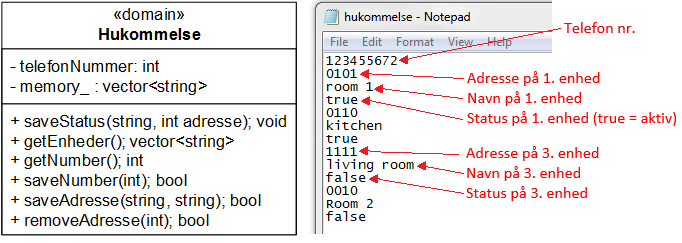
\includegraphics[width=\textwidth]{billeder/uml/PC_dataview}}
     \caption{Hukommelses header og udklip af tekst filen data gemmes i}
     \label{fig:PC_dataview}
\end{figure}


% Implementering - sections af HW og SW

\chapter{Implementering}

% HW implementering

\section{Hardware implementering}

% HW implementering

% SW implementering

\section{Software implementering}

% SW implementering



% Resultater

\chapter{Resultater}

% Resultater



% Resultater

\chapter{Opnåede erfaringer (JS)}

Som en af de første ting kan det nævnes at alle i gruppen har lært og fået erfaringer med at udarbejde større rapporter i Latex hvilket kan blive rigtig brugbart senere hen bl.a. i forbindelse med bachelor projekt.\newline
Vi har som medlemmer, og gruppen som helhed, skulle arbejde noget mere selvstændigt end sidste semester projekt, sammen med at al dokumentation skulle udarbejdes fra bunden. Dette har været med at til give et overblik over sådanne projekters forløb og givet god erfaring med at arbejde struktureret som gruppe. Ydermere har vi haft rigtig god erfaring med at holde korte og konkrete møder, hvor vi hurtigt dannede et overblik over hvor langt vi hver i sær var nået siden sidst vi mødtes, og hvad der skulle fokuseres på ind til næste møde.

% tilføj eventuelt mere individuelt

% Opnåede erfaringer som gruppe

\chapter{Fremtidigt arbejde (SK)}

Et fremtidige arbejde kunne være at udarbejde de dele i projektet som ikke blev nået. Det er at få X10-udtaget til at fungere helt korrekt, samt at få lavet et mere kompakt design af vores print så det kunne implementeres lettere og mere enkelt. 

Lyddetektoren bliver aktiveret ved hjælp af en trykkontakt, et fremtidige arbejde kunne være at færdigudvikle denne. Der skulle laves kredsløbstegninger samt implementering og test. En udvikling af de beskrevet låsemekanismer skulle også udarbejdes for at der kunne leveres et komplet system.

Brugermenuen kunne udvikles med et smartere og mere brugervenlig design. Hvis systemet skulle leveres til andre lande end Danmark ville det være en fordel at der kunne vælges sprog, det gør at systemet kan sælges i større omfang. En App til smartphones kunne laves så der var mulighed for at betjene systemet fra andre steder end hjemme.

% Konklusion

\chapter{Konklusion (PO, SK)}
%Konklusion

Formålet med projektet har været at konstruere et system for at øge børns sikkerhed i hjemmet. Det skulle være muligt at styre bestemt 230Vac udtag i hjemmet, og herigennem låse f.eks skuffer eller kogeplader. Ydermere ønskede vi at modernisere den udbredte babyalarm til en mobil løsning. 

Vi har opnået en prototype, som kan afsende en X10 kommando. PC softwaren, samt CSS hovedenhedens software virker som tiltænkt. Vi har her til slut ikke fået X10-udtagets software til at virke sammen med decoder hardwaren. Vi oplever at den første bit ikke kommer på det tidspunkt den skal, mens resten af bitrækken kommer som ønsket. Dette kan skyldes en langsom opstart i hardwaren eller en software fejl. Prototypen er opbygget på veroboard, dette valg blev taget, da vi oplevede for mange løse forbindelser i fumlebrædderne. 
Det er lykkedes at få systemet til at afsende SMS.  

Samarbejdet har fungeret godt og ud fra gruppekontrakten har gruppen haft et fælles standpunkt og grundlag for projektgennemførelsen. Gennem ASE-modellen er gruppen delt i 2 teams, der har haft hhv. hardware og software som fokuspunkt. Dette samarbejde har fungeret godt, både i de to teams samt gruppen samlet. Gruppen har arbejdet struktureret og professionelt med projektet. Gruppemøderne har spillet en væsentlig rolle for at opretholde strukturen.  

Vi har igennem \LaTeX  oplevet opstartsvanskeligheder, men tilslut er vi rigtigt glade for at have valgt den løsning. 

% Individuel Konklusion

\chapter{Induviduel konklusion}



\section{Bjørn Sørensen}
% Din konklusion her

\section{Jakob Schmidt}
Sammenlignet med 1. semester projektet, så har processen i det her projekt været meget mere struktureret. Sammenholdet og overblikket mellem hvert projektmedlem har været rigtig godt. Det gode samarbejde og overblik skyldes at vi jævnligt har holdt møder, både som selvstændig gruppe, men også sammen med vejleder. Desuden er der afholdt enkelte trivselsrunder, hvor vi hver i sær har skulle fortælle hvordan vi selv følte det gik i projektet. 

Inden vi fik det endelige overblik over hvor omfattende vi kunne lave vores projekt, var det tydeligt at vi havde lidt for stor ambitioner til projektes omfang. Dette blev skåret ned efter første reviewmøde da vi fra anden vejleder blev anbefalet på det kraftigste at revurdere vores use cases.

Personligt har jeg beskæftiget mig med elektroniken i projektet, det kom som narturligt valg da jeg læser på elektro linjen. Fagligt har der været nogle komplikationer med at få de enkelte moduler til at virke som tiltænkt. Projektet har været spændende men samtidig udfordrende, specielt eftersom den nødvendige teori først var helt på plads i den sidste fase af forløbet.  

Overordnet set er jeg rigtig tilfreds med resultatet af vores projekt, på trods af at vi langt fra fik realiseret alle de ting vi havde udtænkt fra første brainstormmøde. Efter revurdering af projektets omfang er alle dele desværre stadig blevet færdige, men ideen er der og de vigtigste dele blev implementeret. 

\section{Jeppe Stærk}
% Din konklusion her

\section{Jesper Christensen}
% Din konklusion her

Semester projektet har budt på mange spændende udfordringer som har gjort det rigtig lærerigt. Vi valgte i gruppen at introducere nogle nye værktøjer til projekt skrivning i LaTeX og en anden Cloud i Github. Det var en lidt hård process i starten da man ikke rigtig kendte programmerne, men i sidste ende har det virkelig givet pote og tror helt sikkert det er noget jeg vil fortsætte med at bruge i kommende projekt forløb.

Vi har i gruppen haft rimelig klare linjer fra starten, omkring hvem der lavede hvad. Vi delte os op i en software og hardware grupper og det synes jeg har været rigtig fint og vi har haft et godt samarbejde i software gruppen og i vores ugentlige møder har vi kunnet følge med i hvad den anden gruppe fik lavet.

At lave software architecturen uden enlig at have kodet noget var en udfordring, men det har været super lærerigt. Synes helt sikkert at jeg er bedre rustet til at lave system arkitektur en anden gang efter at have prøvet krafter med det her. Alt i alt har det været et rigtig godt projekt forløb.

\section{Mick Kirkegaard}
% Din konklusion her

\section{Poul Overgaard}
% Din konklusion her
Jeg er rigtigt stolt af hvad vi som gruppe har opnået i forbindelse med dette semesterprojekt. Det har været en lærerig process, at benytte kurserne tværfagligt og herved opnå ny viden. At arbejde med udgangspunkt i ASE modellen, passer mig fint. Fællesfasen med mange inputs fra gruppen samlet, og herefter en fagspecifik fase, hvor jeg har fungeret som en del af hardware gruppen.  

Personligt har jeg fået stort udbytte af projektet. Vi har som gruppe fra start haft store ambitioner, som vi har måtte forventningsafstemme undervejs grundet tidsmæssigt pres. Grund idéen med vores CSS synes jeg er interessant, og er bestemt et produkt jeg ser vil blive en fast del af hjemmet på sigt.  

Jeg har under møderne, især i projektes sidste fase fungeret som mødeleder/ansvarlig. Det har været rart, at jeg som gruppen yngste og med STX baggrund, har fået lov til at få ansvaret for denne del. Og det er et ansvar jeg gerne tager. Det er bestemt en gruppe jeg kan se mig selv arbejde sammen med igen. 



























\section{Simon Kirchheiner}
% Din konklusion her
Vi har været syv mand i vores projektgruppe, og det har givet os mulighed for at øve os på at samarbejde med flere om et projekt. Vi har været en god projektgruppe med mange forskellige kompetencer, det har medført at man kan hjælpe hinanden godt. Det var en stor fordel at hele projektet var opdelt i faser og havde løbende møder og reviews, så folk ikke bare kørte på helt selv. Faserne har hjulpet med at få et overblik over projektet, og gjort at vi har tænkt over de ting vi skulle lave. I starten af projektet havde vi store ambitioner om at nå mange forskellige ting, men som tiden skred frem måtte vi se i øjnene at det ikke var realistisk. 

I forhold til 1. semester har vi brugt mere tid på at dokumentere det vi skulle lave, og fået en forståelse for de forskellige arbejdsmetoder vi har lært i ISE. Jeg har været på HW delen og der har ASB/MSA fagene givet den nødvendige viden til at kunne løse de problemstillinger vi stod overfor. Jeg tog ansvaret for at skrive logbog/referater, det har givet et godt grundlag for at få struktureret arbejde, da alle kan gå ind i logbogen/referatet og se hvad vi snakkede om.

Vi fik et produkt næsten som planlagt, grundet tidsmangel blev lyddetektoren ikke lavet og vi fik næsten kommunikation over AC nettet til at fungere korrekt. Jeg har fået et stort udbytte ud af dette projekt, og jeg synes vi har haft et godt samarbejde i projektgruppen. Generelt har gruppen fungeret godt og jeg mener vi har et rigtig godt produkt.


% Individuel Konklusion

\include{filer/Underskrifter}

% Litteraturliste
\chapter{Litteraturliste}

\section{Bøger}




\section{Hjemmesider}


\subsection{Opslagsværker}
Generelt C++ opslagsværk \newline
http://www.cplusplus.com [2014-05-24] \newline
UML-light, Finn Overgaard Hansen, Januar 2004 \newline


% Billags-CD struktur
\chapter{Bilags-CD indhold}
Dette er en oversigt over filstrukturen på den vedlagt CD med bilag.

\begin{figure}[!htb]
	 \centering     
     {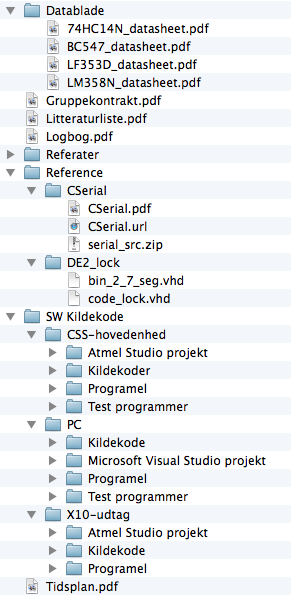
\includegraphics[height=0.7\textheight]{billeder/CD-filstruktur}}
     \caption{Bilags-CD filstruktur}
     \label{fig:PC_package}
\end{figure}

\end{document}
